\documentclass[a4paper, 11pt]{report}
\usepackage{graphicx} % Required for inserting images
% Load the geometry package
\usepackage[margin=2.2cm]{geometry}  % Adjust margins as needed (e.g., 1.5cm, 2.5cm)
\usepackage{hyperref}
\usepackage{tcolorbox}
\usepackage{amsmath}
\usepackage{amssymb}
\usepackage{longtable}
\usepackage{tabularx}
\usepackage{xltabular}
\usepackage{listings}
%\usepackage{glossaries}
\usepackage[final]{pdfpages}
\usepackage[backend=biber, style=numeric, defernumbers=false, sorting=none]
{biblatex}  % Load the biblatex package
\addbibresource{bibitems.bib}  % Point to your .bib file

%\urlstyle{sf}
% Customize the appearance of hyperlinks
\hypersetup{
    colorlinks=true,        % colored links
    linkcolor=blue,         % color of internal links
    citecolor=green,        % color of links to bibliography
    filecolor=magenta,      % color of file links
    urlcolor=cyan           % color of external links
}

\title{Automated Test Selection via ML}
\author{Enric Bassó Xalabardé}
\date{\today}

\definecolor{mygreen}{rgb}{0,0.6,0}
\definecolor{mygray}{rgb}{0.5,0.5,0.5}
\definecolor{mymauve}{rgb}{0.58,0,0.82}

\lstset{ %
  backgroundcolor=\color{white},   % choose the background color
  basicstyle=\footnotesize,        % size of fonts used for the code
  breaklines=true,                 % automatic line breaking only at whitespace
  captionpos=b,                    % sets the caption-position to bottom
  commentstyle=\color{mygreen},    % comment style
  escapeinside={\%*}{*)},          % if you want to add LaTeX within your code
  keywordstyle=\color{blue},       % keyword style
  stringstyle=\color{mymauve},     % string literal style
  frame=single,                    % box it, always
}

\begin{document}

\newpage
\thispagestyle{empty}

\baselineskip 2em


\centerline{\includegraphics[width=0.5\textwidth]{images/URV-logo} }
\centerline{ \includegraphics[width=0.5\textwidth]{images/UOC-logo}}

\begin{center}

\vspace*{1.5cm}

\textsc{Universitat Rovira i Virgili (URV) i Universitat Oberta de Catalunya (UOC) \\
 Master in Computational and Mathematical Engineering\\}


\vspace*{1cm}

\textsc{\Large FINAL MASTER PROJECT }

\vspace*{0.5cm}

\textsc{\large Area: Implantaci\'o de Noves Tecnologies}


\vspace*{1cm}

\textbf{\Large Test selection via Machine Learning }


\vspace{1.5cm}
-----------------------------------------------------------------------------\\
Autor:      Enric Bass\'o Xalabard\'e\\
Tutor:      Jes\'us Ramiro Huguet\\
-----------------------------------------------------------------------------\\
\vspace*{0.5cm}
Barcelona, \today
\end{center}

\newpage

\vspace{1.5cm}
Dr./Dra.  Jes\'us Ramiro Huguet, certifies that the student Enric Bass\'o Xalabard\'e  has elaborated the work under his/her direction and he/she authorizes the presentation of this memory for its evaluation.

\vspace{1cm}

Director's signature:

\pagestyle{empty}
\hfill

\chapter*{FINAL PROJECT SHEET}
\pagenumbering{roman}
\setcounter{page}{1}
\pagestyle{plain}

\begin{table}[ht]
	\centering{}
	\renewcommand{\arraystretch}{2}
	\begin{tabular}{r | l}
		\hline
		Title: & Descriptive of the project\\
		\hline
        Autor: & Enric Bass\'o Xalabard\'e\\
		\hline
        Tutor: & Jes\'us Ramiro Huguet\\
		\hline
        Date (06/2024): & Date of delivery\\
		\hline
        Program: & Master in Computational and Mathematical Engineering\\
		\hline
        Area: & Implantaci\'o de Noves Tecnologies\\
		\hline
        Language: & English\\
		\hline
        Key words & Machine Learning, Neural Networks, Test Automation, Master Thesis \\
		\hline
	\end{tabular}
\end{table}


%%%%%%%%%%%%%%%%
%%% SUMMARY  %%%
%%%%%%%%%%%%%%%%
\chapter*{Abstract}
\addcontentsline{toc}{chapter}{Abstract}

In the landscape of modern software development the need for rapid releases without compromising quality is fundamental to competitive development and reliable production. This thesis explores the implementation of a machine learning application for automated test selection, aiming to to improve the efficiency and accuracy of software testing process. The proposed solution uses a Neural Network with a Natural Language Processing layer, in order to adapt to changing code bases and dynamically react to currently perceived status of the environment. This project presents an overview to the theoretical foundations of machine learning and neural networks to elaborate on their application on the developed software. Those foundations are used to build and program the components, which include the neural network architecture via the library PyTorch, the integration of the Natural Language Processing layer and the creation of an API to allow high-level interaction from a user. The effectiveness of the tool is demonstrated with example tests that highlight its flexibility and learning capability with a variety of data. We show that the tool is able to guess the relevant test functions for a given method, and the correct choices are in top 33\% ranking of guessed relevance over 98\% of the time. Furthermore, this work not only addresses the technical side of the development, but also the project management considerations, such as risk assessment, budget estimation and project management deliverables. This presents a global view of the process of implementation of new technologies for software engineering.
\vspace{1.5cm}

\textbf{Keywords}: Machine Learning, Neural Networks, Test Automation, Master Thesis, Software Development, PyTorch, Natural Language Processing.
\tableofcontents
\listoffigures
\listoftables


\chapter{Introduction} \label{Section: Introduction}
\pagenumbering{arabic}
\setcounter{page}{1}
\pagestyle{plain}
\section{Background}
The standards of modern software development have led to the need for faster and faster releases while keeping software quality. This increasing pace is driven by the competitiveness of the market, where a speedy delivery can play a crucial factor to a product's success. To comply with these standards, software development must be tested against an ever-growing number of requirements, including functionality, security, performance, compatibility and reliability of the product developed.

The complexity and scope of the testing can become increasingly challenging for a growing project. The manual and semi-automated testing methods are usually slow and resource-intensive\cite{Mandic2023Test}, resulting in bottlenecks that can delay development, and can also divert resources an effort from the development itself.\cite{LAUWAERTS2024Test}

In response to this, we propose the creation of an automated testing tool with adaptive capabilities powered via Machine Learning (ML). This application will be designed to streamline the testing process, i.e. continuous integration, regression and unit testing tasks, reducing the time and effort required. The AI layer will enable it to dynamically adjust itself to its environment, and will ensure that the tests can be prioritised by relevance to a given scenario, especially if resources needed for execution are scarce.

The ultimate aim of this implementation is automating repetitive and time consuming tasks, and enabling development teams to focus on further expanding their product quality.

\section{Challenges}
Generally speaking, most of the testing has to be conducted, or at least set up, manually. The process can become time-consuming, error prone and resource-intensive.

Manual testing makes it difficult to keep a rapid pace of development due to the changes in the codebases. As a development team integrates new features and updates, the testing suite must be update in accordance. This is likely to induce errors, especially in time-constrained environments.

Therefore, an automated approach to test selection can streamline these necessary but repetitive steps, particularly in situations speed and efficiency are needed, reducing the likelihood of human error and freeing up resources.

\subsection{The case for automation and ML}
The rationale behind our idea is to exploit AI automation to address the challenges that arise from the dynamism needed for testing. We target the creation of a tool that can provide quick, reliable and intelligent identification of relevant tests, and by extension, issues throughout the development process.

AI allows for great adaptability, and for natural adjustment during the lifetime of the project by learning from the latest data in the project. This would allow the application to develop together with the project, and adapt to new introduced features.

The main focus of this application is to accelerate the and prioritise integration, regression or unit tests in response to code changes, and provide real-time feedback for developers. It should become part of the continuous integration and delivery pipelines.

\section{On the Nature of this project}
This project is a master thesis. It has a technical side, which includes the theory, and practical implementation of a solution, followed by an analysis on results achieved. But it is not its only focus. \textbf{This work is intended to be a representation of a real project, which implies project management considerations}, including the task planning, the budget, the risk analysis and the project deliverables. Therefore there is an entire section devoted to this side of the thesis. The project management part will also be summarized in the Project Deliverables, attached on Appendix~\ref{Apx: Project Deliverables}. The planning of this project has been integrated within the project management section.

\section{Approach}
As mentioned\textbf{, this project has a secondary focus as a project management report.} Through this management layer we will define deliverables and account for changes and progress of the plan.

On technical side it will be handled like a software development project, with a very straightforward procedure. First we will select the tools to be used. Then a progressive implementation of the devised features will take place, adjusting and analyzing the remaining ones within the context of the project. The implementation will be based on properly researched literature and theory (presented extensively in Chapter~\ref{Theory}). This process might require re-assessing the objectives and evaluating progress based on remaining time (budget), feasibility of the remaining work and risks triggered during the process. Hence, the objectives and planning might be subject to change as the project evolves.

Lastly, when the implementation has executed to a satisfactory degree, we shall attempt a practical example showcase of the implemented functionality, followed by an analytical evaluation on the performance and the results achieved.

\section{Document Structure}
The document is structured to provide a comprehensive overview of the project, from its start to its final deliverables.

It begins with the project introduction, detailing the background, challenges, and the rationale for the proposed solution (Section~\ref{Section: Introduction}).
We follow with a project management report, including the timelines, cost estimates, risk assessments and objective planning (Section~\ref{Project Management}).
Then we present the theoretical foundation of the concepts used in the implementation (Section~\ref{Theory})).
The final sections show an example implementation of the application, and analyze its efficiency and results (Section~\ref{Section: Methodology} and Section~\ref{Implement: Practical}).
Finally, conclusions and outlook will be presented in the last section (Section~\ref{Conclusions}).
The appendices contain more detailed information about some design decisions, explaining the problems that motivated them. They also contain information on document revisions throughout the project, and a more detailed project monitoring report based on the project management section presented in the form of standard project management templates..

Each section is designed to offer clear and detailed insights into different aspects of the project.

\chapter{Project Management}\label{Project Management}
The purpose of this section is to present a business case for the development and implementation of an automated tool to enhance a testing facility. The aim is to improve the efficiency and quality of software by reducing the time and resources required for regular testing of assets present in the facility.

Following the motivation exposed in Section~\ref{Section: Introduction} we define our objectives and expected benefits, and present a plan for its implementation.

\section{Objectives and potential benefits}\label{Intro:Objectives}
We aim to produce an application which is able to identify relevant tests for a given codebase, and to process train and learn in a dynamic fashion. Adoption of the produced tool in a given codebase is intended to:
\begin{itemize}
    \item Improve software quality: Detecting and identifying potential problems in the project in a timely manner and properly addressing them ensures a more robust and dependable product.
    \item Accelerate development: Automating the testing step should reduce the time needed for releases and facilitate a more agile development of any project.
    \item Resource optimization: Reducing the amount of time and effort dedicated to testing by delegating it to an automated tool will allow for more intense focus on the development itself, while simultaneously reducing the human error-proneness of the process.
    \item Adaptability through AI: Incorporating an AI layer will enable our tool to dynamically adapt to changes in the code base and keep itself up-to-date with the current state of the project. Learning from historical data could keep the tool robust in its environment while enabling it to integrate to other existing environments as well.
\end{itemize}

Achieving the aforementioned objectives will lead to the following benefits:
\begin{itemize}
    \item Better quality product: Reducing error proneness and bugs will make for a better product and therefore.
    \item Better cost to benefit ratio: A faster development process will allow businesses to get their products to market sooner while reducing development process costs.
    \item Higher sustainability: If the tool is successful, it can minimize the amount of testing needed according to the situation at hand. In large projects this can significantly impact resources expenditure, in the form of computational time, en by extension, energy consumption.
    \item Better developer focus: Automatising this kind of tasks can free up time for developers to work on other parts of the project. Besides the increased efficiency, this also has a positive impact on developers as testing processes are known to be tedious.
\end{itemize}

Summarizing, the automated testing tool will provide a number of benefits to businesses, including improved software quality, reduced costs, accelerated development cycles, and reduced human error.

\section{Impact on sustainability}
An automated testing tool is designed for resource optimization. As such, this would naturally reduce the energy consumption of manual testing processes.

Furthermore in very large project, where running testing suites might cumulatively incur in a large cost in terms of time, effort and energy consumption, the application might help prevent unnecessary tests from executing, saving up on those resources. This might be inconsequential for average projects, but in truly massive projects this difference cannot be understated.

\section{Focus and methodology} \label{Methodology}
We suggest a traditional waterfall approach to project methodology:

\begin{itemize}

\item  Design Phase
\begin{itemize}
\item  \textbf{Subtask 1}: Define Requirements
\item  \textbf{Subtask 2}: Define Application components
\item  \textbf{Subtask 3}: Select applicable tools (coding language, external libraries,...)
\end{itemize}

\item  Development Phase:
\begin{itemize}
\item  \textbf{Subtask 1}: Core Feature implementation
\item  \textbf{Subtask 2}: Implement AI capabilities
\item  \textbf{Subtask 3}: Add NLP capabilities
\item  \textbf{Subtask 4}: Core components Testing
\end{itemize}

\item Fine-tuning and Refining
\begin{itemize}
\item  \textbf{Subtask 1}: Provide an API interface
\item  \textbf{Subtask 2}: Produce a simple interface to minimize user input needed to make use of the application.
\item  \textbf{Subtask 3}: Provide the application with report generation capabilities for performance checking.
\end{itemize}

\item  Deployment Phase:
\begin{itemize}
\item  \textbf{Subtask 1}: Conduct rigorous testing. Performance indicators:
    \begin{itemize}
        \item \textbf{Integration Tests Results}: Regularly check that different parts of the system work together as intended. Assess success rates and identify any inconsistencies or failures in integration tests, ensuring comprehensive coverage of critical system interactions.
        \item \textbf{AI Performance Metrics}: Evaluate the AI layer's performance using metrics such as accuracy, precision, recall, and F1 score. Confirm that the AI adapts to changing codebases, learns effectively from historical data, and reliably identifies potential issues in the software.
        \item \textbf{Performance Evaluation}: Verify that the automated testing tool does not cause issues or bottlenecks in the existing system or the development roadmap. Monitor response times, resource utilization, and system stability to ensure optimal performance without hindering the overall workflow.
        \item \textbf{Usability }: Assess the user-friendliness of the tool through usability testing. Collect feedback from potential end-users to ensure that the tool is intuitive and easy to use.
        \item \textbf{Reliability Testing}: Evaluate the reliability of the automated testing tool by assessing its ability to consistently produce accurate and dependable results. Identify and address any instances of tool malfunction or unexpected behavior.
    \end{itemize}
\item  \textbf{Subtask 2}: Generate application Documentation
\item  \textbf{Subtask 3}: Produce a user Manual to deliver together with the application.
\end{itemize}
\end{itemize}

\subsection{Approximate time distribution per task}
The plan here presented is now the final iteration. The plan has been reworked and re-assessed several times in the course of the project. This also acts as en effective summary to the tasks undertaken in this thesis.
The tasks have been summarized in Tab.~\ref{Tab:Effort Projection}. This planning also serves as an outline for the budget estimation, as the time invested has been equated to the budget cost (as in a real case scenario, where a budget can be measure in man/hours).

\begin{table}[ht!]
\centering
\begin{tabular}{|l|c|}
\hline
\textbf{Phase} & \textbf{Total Time (h)}  \\
\hline \hline
\textbf{Phase 1: Planning}  & \textbf{86}  \\
\hline
   Decide on a topic and objective  & 30  \\
\hline
   Write Plan and Project Charter  & 28  \\
\hline
  Define Technical Requirements  & 28  \\
\hline \hline
\textbf{Phase 2: Core Development}  & \textbf{190}  \\
\hline
   Core Feature Implementation  & 70  \\
\hline
   Implement AI layer  & 60  \\
\hline
   Implement NLP layer  & 40  \\
\hline
   Core Testing and fixing  & 20  \\
\hline \hline
\textbf{Phase 3: Refinement}  & \textbf{166}  \\
\hline
   Fine Tuning and bugfixing  & 80  \\
\hline
   Implementing multi-class Input Handling  & 20  \\
\hline
   Implement API  & 30  \\
\hline
   Implement Logging layer  & 10  \\
\hline
   Implement Reporting feature  & 6  \\
\hline
   Implement Multi-class output handling  & 20  \\
\hline \hline
\textbf{Phase 4: Deployment}  & \textbf{50}  \\
\hline
   Rigorous Testing of the Application  & 20  \\
\hline
   Documenting the Application  & 10  \\
\hline
   Technical Report  & 10  \\
\hline
   User Manual for the Application  & 10  \\
\hline
\end{tabular}
\caption{Approximate time dedicated to each projected task.}
\label{Tab:Effort Projection}
\end{table}

The tasks outlined in the table have also been represented in a Gantt chart in Fig.~\ref{fig:Gantt_plan}. The gantt chart has been elaborated under the assumption that in average the developer will have about 14 hours per week of dedication to the project.

\begin{figure}[ht!]
    \centering
    \includegraphics[width=0.99\textwidth]{lastchart.png}
    \caption[Estimated time investment per task]{Estimated tasks and time investment projected in a Gantt chart as expressed in the table. Tasks colored in green are complete. Holidays during which work was suspended are highlighted in light Blue.}
    \label{fig:Gantt_plan}
\end{figure}


\section{Cost of the project}
The cost of this project is presented in man/hours. To reach the following figures the estimations of the Gantt plan in Fig.~\ref{fig:Gantt_plan} were used. As mentioned, based on a simple conversion considering the theoretical time dedication that is required of this project and considering that is done by a single person. Each week has been counted to be approximately 14 man-hours dedication

\begin{table}[ht!]
\centering
\begin{tabular}{|l|c|}
\hline
\textbf{Phase} & \textbf{Total Time (h)}  \\
\hline \hline
\textbf{Phase 1: Planning}  & \textbf{86}  \\
\hline \hline
\textbf{Phase 2: Core Development}  & \textbf{190}  \\
\hline \hline
\textbf{Phase 3: Refinement} & \textbf{166}\\
\hline \hline
\textbf{Phase 4: Deployment}  & \textbf{50}  \\
\hline \hline
\textbf{Total} & \textbf{492} \\
\hline
\end{tabular}
\caption{Total cost of the project estimated from the time effort that each task requires.}
\label{Tab:Budget}
\end{table}

Straying from the budget allocation will be considered as triggering a risk case scenario.
\clearpage
\section{Risk assessment}
The risks are categorized in different types, with a keyword acronym and a numeric identifier:

\begin{itemize}
    \item IM-xxx: Implementation Difficulty
    \item AI-xxx: AI-related problem
    \item IN-xxx: Integration problem
    \item BU-xxx: Business problem
\end{itemize}

\begin{xltabular}{1.0\textwidth}{|c|X|c|c|X|}
\hline
\multicolumn{1}{|c|}{\textbf{Risk}} & \multicolumn{1}{c|}{\textbf{Description}} & \multicolumn{1}{c|}{\textbf{Probability}} & \multicolumn{1}{c|}{\textbf{Impact}} & \multicolumn{1}{c|}{\textbf{Mitigation Strategy}} \\
\hline
\endhead
\multicolumn{5}{|r|}{{Continued on next page}} \\
\hline
\endfoot
\endlastfoot
\centering
    IM-001 & The automated testing tool proves difficult to implement in the given timeframe & High & High & Either the project is unfeasible or the scope is unattainable. \\
    \hline
    IM-002 & The implementation might be too difficult to be made practical as an API & High & Medium & No API can be implemented in a realistic timeframe. Present application as prototype. \\
    \hline
    IM-003 & A generic capability to schedule and run tests in a codebase might be too difficult to implement & High & Medium & No automatic implementation of automatic process launching can be implemented as part of the tool. Will require user to post-process \\
    \hline
    IM-004 & A compact GUI might be difficult to achieve with the current level of expertise. & Low & Low & Downgrade the GUI to a simple library interface for use in-code.\\
    \hline \hline
    AI-001 & The AI capabilities might not work as intended or be too difficult to implement & Medium & High & The AI layer might prove unfeasible to implement. Choose a simpler tool or algorithm. \\
    \hline
    AI-002 & AI might not be as useful as anticipated to the problem & Medium & High & Change the scope of the tool applicability \\
    \hline \hline
    IN-001 & The automated testing tool may not integrate seamlessly with existing systems and processes. & Medium & Medium & Define clear integration requirements and specifications (i.e restrict input data formatting). \\
    \hline
    IN-002 & The tool might be too difficult to test in a live scenario. & Medium & High & A proper scenario should be developed in which to properly and extensively test the tool. \\
    \hline
    IM-003 & Generating datasets that make sense for the training of the tool for a performance analysis might be too difficult to achieve in the given timeframe. & Medium & High & Use simplified datasets to minimally validate the tool or accept a narrow testing frame on which to expand at a later date.\\
    \hline \hline
    BU-001 & The automated testing tool may not achieve the desired business objectives, such as improved software quality, reduced testing costs, and accelerated development cycles. & Low & Medium &  Reassess objectives if necessary with adequate continuous monitoring of the progress.\\
    \hline
    BU-002 & The allocated time to the project was not enough to achieve objectives & Medium & Medium &  Increase the the allocation and effort to the project. This will imply an increase in cost. \\
    \hline
    \caption{Risk Control Table. Version 4.0}
    \label{table:Risks}
\end{xltabular}


\section{Deliverables}
In this section we discuss the deliverables. There are two kinds of deliverables: The Project Deliverables and the Technical Deliverables.

Considering the risks triggered (see Appendix~\ref{apx:Project Monitoring}), the deliverables have been re-defined along the project, and those presented here are the final iteration.
For the project deliverables, we aim to deliver a set of focused summaries:
\begin{itemize}
    \item A project charter a
    \item Planning report
    \item Risk report
    \item Budget report.
    \item Objective modification report
    \item Project closing report
\end{itemize}
The finalisation of the technical project aims to deliver:
\begin{enumerate}
    \item A functional automated testing tool with an AI layer. It should be able to:
    \begin{itemize}
        \item Generate a trained utility (a Neural Network) tailored to the case at hand.
        \item Correctly relate an input to a given set of outputs (e.g. match a method name to a corresponding, known test function).
        \item Generate reports on training and performance.
        \item Offer mechanism for utility persistence (save and load the Neural Network).
    \end{itemize}
    \item An API that simplifies the application's use for an end user. It should be integrated as part of the tool. It should be able to:
    \begin{itemize}
        \item Allow configuration the tool for different needs i.e: codebase size.
        \item Generate reports of actions taken during execution.
        \item Seamlessly execute the functionality of the tool in the simplest form possible from a user point of view.
    \end{itemize}
    \item Documentation on the functionality and usage of the tool for end user recipients.
    \item A consolidated report on project progression and technical implementation.
    \item An example implementation to serve as an example for users.
\end{enumerate}

\subsection{Communication Plan}
    The project is a development of a software tool. During a the development phase of this project, regular meetings were scheduled with the receiver of the tool (the client) to create a communication channel that allows feedback into the development.

    Ultimately, the communication focus of the tool should be its documentation. It will be enclosed in the code of the API itself, ideally providing enough information and clarity through the use of the python self-documenting capability (class and function docstrings).  This documentation has also been processed and encoded in a deliverable package in html.

    In the long term, users can provide feedback for the enhancement and further development of the tool based on the needs that arise from frequent usage.

\subsection{Execution  Progress}
    Technical summary of the current capabilities. For an in-depth explanation, please see the corresponding technical report Section~\ref{Section: Methodology}
    \begin{itemize}
        \item The tool has been coded in its full projected core functionality. It can:
        \begin{itemize}
            \item Created an API library to interface with the application as simply as possible.
            \item Generate a Neural Network object using the \textit{PyTorch} library using a simple set of function calls and configuration parameters.
            \item Configure an arbitrary number of inputs and choose the outputs given a configured dataset in the form of a Pandas DataFrame object.
            \item The inputs can be encoded and one-hot vectors, or processed through a layer of Natural Language Processing (NLP).
            \item The targets can also be encoded in the NLP embedding before running the comparison with the neural network outputs.
            \item Learn from data from a pandas DataFrame.
            \item Different targets for stopping the training can be configured.
            \item Classify an input into a set of output labels (multilabel classification).
            \item Validate the learning progress by evaluating the correctness of solutions vs a validation dataset.
            \item Generate a set of output logs for tracking the application process. It generates human-readable logs and programmatically-parseable logs (in the form of a jsonl formatted file).
            \item Generate a live plot of the training process and save it at the end of training for assessment a posteriori.
            \item Create the relevant documentation for the modules and functions in the application in the form of an html navigable directory.
            \item Save and load trained Neural Networks from memory.
        \end{itemize}
        \item Cancelled objectives:
        \begin{itemize}
            \item Creating a Graphical interface to display the use and results of the tool (lack of time).
            \item Creating a User Manual to guide a new user step by step in the usage of the application (lack of time).
            \item Test scheduling automatisation layer (unfeasible unless very specific assumptions about the environment of deployment are made).
            \item Multi-class output classification (unproductive for the scope).
        \end{itemize}
    \end{itemize}

    By comparison with the projected plan, we claim our progress is falling short of the projected objectives. Final delivery status evaluated under 100\% due to shortcomings of projected features.
    $$
    \boxed{\text{Execution Progress} = 90\%}
    $$


\chapter{Technical Foundation}\label{Theory}
In this section we present an overview of the theoretical concepts that will be used in the implementation of the application.

We need to present the concepts of Machine Learning (ML), Neural Networks (NN) and Natural Language Processing (NLP) through embeddings. Following the theoretical foundation, we need to delve into the particular use of the libraries that will serve as building blocks of our software implementation.

\section{Machine Learning}
ML  is a subset of AI based on the implementation of algorithms that make predictions based on existing data.

An ML Algorithm will use the data to train and learn patterns with the primary goal of extrapolating them to unseen data, and hopefully result in a correct result (a prediction). A successful implementation of a ML will allow the automation of tasks that usually require human intelligence to execute
.
\subsection{The origins of Machine Learning} \label{Theory: ML}
The first mention to the terms ``Machine Learning" appear in a 1959 paper by Arthur Samuel \cite{samuel1969_ML_origin}, in which he tried to produce a program that learned to play the game of checkers and improved its performance over time, ending up a better player than the person who programmed it.

Since that first paper, ML has been an attractive field of development, but the computational power at the time severely limited what could be achieved with it. However in the decades that followed it was already explored for its potential in different fields, like medicine~\cite{Shortliffe1977_ML_medicine} (Shortliffe, 1977) or chemistry~\cite{Lindsay1980_ML_chemistry80} (Lindsay, 1980). The study and development of algorithms that nowadays are the cornerstone of ML were also researched before the current explosion of popularity of ML and AI, such as the k-means algorithm~\cite{MacQueen1967_Methods_Multivariate} (MacQueen, 1967) and genetic algorithms~\cite{Holland1992_Genetic_Alg} (Holland, 1992) and even the beginning of the rise of neural networks~\cite{Rumelhart1986_Backpropagation} (1986).

With the improvement of computational power in the last decades, the field of ML has expanded exponentially, especially with the increasing popularity of AI applications. Many approaches and varieties have been developed leading to rapid breakthroughs in many fronts. From image classification~\cite{Krizhevsky2012_AlexNet} (Krizhevsky, 2012), game playing~\cite{Silver2016_Go}(Silver, 2016) or Natural Language Processing~\cite{vaswani2023_Attention}(Vaswani, 2017).

This has brought ML to the forefront of not only the academic world but to many other fields, with groundbreaking applications such as chatGPT~\cite{GPTopenai}.

\subsection{Core Concepts of ML}
Broadly speaking, a ML algorithm is an iterative process in which a set of parameters is adjusted to better fit to an expected result. A vast array of concepts and approaches come into play depending on the problem or infrastructure at hand, but machine learning can be categorized into three types: supervised learning, unsupervised learning, and reinforcement learning.

\begin{itemize}
\item \textbf{Supervised Learning}: This approach involves training a model on labeled data, where each training example is paired with an output label. The algorithm attempts to make its output as close as possible to the target label. Common algorithms include linear regression, logistic regression, support vector machines (SVMs), and neural networks. The model learns to map inputs to outputs, making predictions for new, unseen data. This is the type of learning used in this work.

\item \textbf{Unsupervised Learning}: In unsupervised learning, the model is given data without explicit labels. The goal is to uncover hidden patterns or intrinsic structures within the data. The algorithm attempts to group similar data points together, or reduce the dimensionality of the data to highlight relevant patterns. Algorithms such as k-means clustering, hierarchical clustering, and principal component analysis (PCA) are commonly used.

\item \textbf{Reinforcement Learning}: This type involves a model that learns to make decisions by performing actions under a system of penalty-reward.  The algorithm attempts to maximize the cumulative reward over time by learning the most effective strategies through trial and error. In this case algorithms are highly problem-specific.
\end{itemize}

Each of these approaches has unique strengths and applications, contributing to the flexibility of ML as a concept.  The next section will focus on the particular case of neural networks, discussing their architecture, training mechanisms, and the innovations that have driven their success in various AI applications.

\section{Neural Networks}\label{Theory: NN}
In this section we will see how neural networks have revolutionized the field, offering unparalleled capabilities in pattern recognition and predictive modeling. Neural networks are inspired by the human brain, consist of interconnected layers of nodes or "neurons". The data gets introduced to the network as a numerical input, and propagates through layers (sets of neurons) until an output is reached after the last. These networks have demonstrated exceptional performance in various applications, from image and speech recognition to natural language processing and beyond.

\subsection{The origins of Neural Networks}
The concept of neural networks dates back to the 1940s when Warren McCulloch and Walter Pitts introduced a mathematical model of artificial neurons in their seminal paper ``A Logical Calculus of Ideas Immanent in Nervous Activity''~\cite{McCulloch1943_Calculus_nervous}. This model laid the foundation for Artificial Neural Networks (ANNs), proposing that neurons could be combined to perform logical operations.

In the 1950s and 1960s, Rosenblatt developed the \textbf{perceptron}~\cite{Rosenblatt1958_Perceptron}(1958), a type of neural network for binary classification. Originally this was received with great optimism with the perspective that the perceptron could evolve to a proper full-fledged machine consciousness~\cite{NYT1958}\footnote{This is not an academic article, but it shows the mindset of the time}. Despite initial enthusiasm, the limitations of the perceptron, as highlighted by Minsky and Papert in their book ``Perceptrons'' (1969)~\cite{Minsky1969_Perceptrons}, led to a temporary decline in neural network research.

The re-emergence of neural networks in the 1980s came with the introduction of the backpropagation algorithm by Rumelhart, Hinton, and Williams (1986)~\cite{Rumelhart1986_Backpropagation}. This algorithm allowed for the efficient training of multi-layer neural networks, overcoming the limitations of single-layer perceptrons. The development of more advanced architectures and training techniques in subsequent decades has significantly expanded the capabilities of neural networks. Innovations such as convolutional neural networks (CNNs), recurrent neural networks (RNNs), and, more recently, transformer models have enabled breakthroughs in many fields fields, like image recognition, natural language processing, and game playing, as explained above in Section~\ref{Theory: ML}. These advancements have been facilitated by the availability of large datasets and increased computational power, leading to the modern era of ML and AI, in which varieties of NN are one of the most flexible widely used implementations.

\subsection{Neurons and Layers of a Neural Network}

As it has been stated, a NN relies on a system of neurons (entities with an input value and an output value), and layers (sets of neurons).

First, an input is given in numerical form to the first layer, or \textbf{input layer}. This numerical form needs to represent the input. It can be a set of numbers, or binary values, or another abstraction that the implementer decides on. Each of the neurons that receives an input, will forward it to its output. This is true for all neurons in the NN.

Each output is directed to the next layer. Between each pair of neurons, a link is established, such that the output of the previous one becomes the input of the following one. This link has an associated function (a weight and/or bias), that modifies the value going through it before it reaches the next neuron. This process continues until the last layer, or \textbf{output layer}, is reached, and all the value coming out of this layer become the outputs of the NN. To perform this action, is to perform a \textbf{forward pass through the NN}. Any layer between the input layer and the output layer is called a \textbf{hidden layer}, which are named like this because the values going through them are not directly observable, unlike the input and output layers.

Then, when an input is given to the input layer, and a forward pass is executed, we can evaluate its outputs against some targets. Using the backpropagation algorithm, the gradients of all parameters (weights and biases) involved can be used to estimate a change on them such that the output will become closer to the target. This is what it means for a NN to learn, or to be trained.

A NN can become arbitrarily complex. The most straightforward increase in complexity of the NN can be simply adding neurons and hidden layers, but other changes are possible, such as different type of layers, or intermediate steps of data processing (e.g., normalization of the data between layers or dropout techniques). This structure is what we refer to as the \textbf{architecture} of the NN. The more complexity we add, the more complex the patterns and relationships that can be learned. The popular term ``deep learning''~\cite{LeCun2015_DeepLearning} (LeCun, 2015) refers to having a large number of hidden layers, so a NN can learn complex patterns and relationships. However, the complexity of NN has to be scaled carefully. More complexity does not immediately mean more capability, as an overly complex model is not without other risks (see Section~\ref{Theory: NN-shortcoming}).

The ability of a NN to learn is heavily problem dependent, and unfortunately there is no clear rule of thumb to designing an optimal architecture. Most implementations will require a good deal of trial and error, turning the architecture design of it into an iterative process until a satisfying one is found. For the sake of reference in our implementation later, a few types of layers and techniques will now be briefly presented.

\subsection{Layer types}
Neural networks can have different types of layers, with each being suitable for different types of data and tasks. The choice of layer type is crucial for designing effective neural network architectures. This section explores the most common types of layers: Linear Layers, Recurrent Neural Network (RNN) Layers, Convolutional Neural Network (CNN) Layers, and other specialized layers.
\subsubsection{Linear Layers}\label{Theory: Linear layers}
 Linear layers are the most straightforward and common type.  In a linear layer, the input gets processed via a linear function. Mathematically, the output of a linear layer can be expressed as:

 $$y=Wx+b$$
 where x is the input vector, W is the weight matrix, and b is the bias vector.

 These layers are commonly used in for all types of NN. If each of the layer's neurons are connected to all of the neurons of the following layer, we speak of either a \textbf{Fully Connected} (FC) layer or a dense layer. This massive number of links is what allows complex patterns to emerge. Nevertheless this type of layer is actually limited in terms of the complexity it can learn, given that all relations it models can only be linear. Some techniques can be applied to the data flowing through the layer in order to introduce some effects that would allow to capture non-linear patterns, like an activation function, which will be presented below.

\subsubsection{Convolutional Layers}\label{Theory: CNN layers}
 Convolutional Neural Networks (CNN) are designed to work with spatial data (e.g. data has associated coordinates). CNN layers apply convolutional operations to the input, using filters (or kernels) that produce feature maps. The expression for a basic CNN:

\begin{equation*}
    y(i,j) = \sum_m{\sum_n{W(m,n) \cdot x(i+m, j+n}) + b(i,j)}
\end{equation*}

 Where $x$ is the input,$W$ is the filter, $b$ is the bias and $y(i,j)$ is the output at position $(i,j)$ (associated coordinates).

 CNN can use their dependency on associated coordinates  to learn spatial hierarchies or local patterns and features of the input data, hence their application in image recognition, optical character recognition (OCR) or more advanced features like videos.

 The main idea of CNN is to produce a mapping out of different regions of the original input (e.g. different areas of an image), and process them using the filter. Each of them produces a mapping (called a plane of the convolution), and those can later can be further processed. CNN layers are typically followed by pooling layers, which reduce their dimensionality to make the model more computationally efficient, at the cost of some precision. However, one can try to maximize the captured variance with the remaining dimension, for example through PCA analysis, therefore retaining as much of the information as possible.

 Since their introduction~\cite{Atlas1987_Phoneme}(Atlas, 1987), and early use~\cite{LeCun1989_Handwritten_Zip} (LeCun, 1989) they have been deeply studied and experimented on. Their effectiveness was proven by recognizing handwritten documents~\cite{LeCun1998_Doc_Recognition}(LeCun, 1998) and after that their usage continued to expand, with applications being central to impactful highlights in the recent history of AI. CNN was the subject of the influential paper on AlexNet~\cite{Krizhevsky2012_AlexNet} (Krizhevsky,2012) and the VGG~\cite{Simonyan2015_Deep_Convolution} (Simonyan, 2015), both breakthrogh papers in the field of image recognition tasks.

\subsubsection{Recurrent Neural Network Layers}\label{Theory: RNN Layers}
 Both linear layers and CNN layers are \textbf{feed-forward Neural Networks}, meaning that the neurons connect only to the neurons in the following layers. However, there is another kind of NN. The cases in which neurons can be connected to other neurons in the same or previous layers are called Recurrent Neural Networks (RNN).

 RNN layers are designed for sequence data, such as time series, text, and speech. Unlike feed-forward layers, RNN layers have connections that form cycles, creating an effect of persistence from previous forward passes. Thanks to that, they are suitable for NLP processing, especially when the sequential context is important (e.g a full cohesive text).

 There are different kinds of RNN, the most simple one being the Elman layer~\cite{Elman1990_Structure_Time}(Elman, 1990):
\begin{equation*}
    h_t = \sigma_h\left(W_hx_t+U_hh_{t-1}+b_h\right)\\
\end{equation*}
\begin{equation*}
    y_t = \sigma_y\left(W_yh_t+b_y)\right)
\end{equation*}

 Where $x_t$ is the input, $h_t$ is the result of applying a hidden layer to the input and $y$ is the output vector. $W$, $U$ and $b$ are parameters associate with each operation (weights and biases). $\sigma$ represents an an activation function. In this equation, the $t$ subindex refers to time units, or simply passes to the network, and we can see how $h_{t}$ depends on $h_{t-1}$. This means whatever passed through the NN will have a lasting effect on all subsequent passes, hence the effect of persistence is achieved. This is how the NN might be able to process a given input (e.g. a sentence) while being influenced by previous already-processed input (e.g. preceding context).
 Other variants have emerged with slight variations and varying degrees of additional complexity, like the Long Short-Term Memory (LSTM) layer~\cite{Hochreiter1997_LSTM} (Hochreiter, 1997) or the Gated Recurrent Unit (GRU)~\cite{Cho2014_GRU} (Cho, 2014) among others. They aim to solve some problems (most notably the vanishing gradients problem, see Section~\ref{Theory: NN-shortcoming}), but the principle remains the same.

\begin{figure}[ht!]
    \centering
    \includegraphics[width=0.32\linewidth]{Rumelhart_LNN.png}
    \includegraphics[width=0.25\linewidth]{Elman_NN.png}\\
    \includegraphics[width=0.49\linewidth]{Lecun_CNN.png}
    \caption[Sketches of NN]{Sketch of each layer type as presented in their respective papers. Top left: Linear Layer~\cite{Rumelhart1986_Backpropagation}(Rumelhart, 1986). Top right: RNN~\cite{Elman1990_Structure_Time}(Elman, 1990). Bottom: CNN~\cite{LeCun1998_Doc_Recognition}(LeCun, 1998)}
    \label{fig:layers Sketch}
\end{figure}
\subsubsection{Other Layers}\label{Theory: Other layers}
The usage of the aforementioned layers is not exclusive. NN can have architectures joining different layers, in an attempt to apply different techniques and capturing different features of the input data. For instance it is common to have a NN recognizing images be composed of CNN layers followed by linear layers.

But those aforementioned layers are not the only ones in use. Other types are also exist, and not all of them accomplish the same purpose of capturing data or learning patterns, but rather they can also execute other operations on the data passing through. The most common types are simply intermediate operations, for example data normalization.

\begin{itemize}
    \item \textbf{Activation Layers}: They execute a function that scales the output out of the previous layer. They are named activation because they can control if a certain output propagates or not. They depend on an activation function. The use of activation layers is very flexible. Here are some common examples:
    \begin{itemize}
        \item Linear Unit (Lu): Simply applies a linear function to the values going through.
        \item Rectified linear unit (ReLu): Applies a linear function to the values going through, but returns 0 if the value is below 0. This is intended to train a NN to recognize non-linear relationships.
        \item Leaky Rectified Linear Unit (LeakyReLu): Same as ReLu, but instead of returng a 0, returns a linear function with a small slope. The idea is still to capture non-linear relationship like with a ReLu, but the small slope should prevent gradient problems that can de-stabilize the learning process.
        \item Sigmoid: A sigmoid is a re-scaling function that takes any number $\in \mathbb{R}$ and maps it to the range $(0, 1)$. This is useful if we want to interpret values as independent probabilities.
        \item Softmax: The softmax function re-scales all inputs to the range $(0,1]$, in such a way that their sum add up to $1$. This is useful if we want to interpret a set of values as a probability distribution.
    \end{itemize}
    \item \textbf{Normalization Layers}: They normalize the data going through them. This is useful in cases where the magnitude of the data might not be as signficant as other features (e.g. relative size), and executing this step help stabilize the iterative process, for example preventing the numerical values of a gradient from being too big, or too small, which could cause problems in the optimization step.
    \item \textbf{Pooling Layers}: They combine execute a reduction in dimensionality. This is useful to reduce the amount of data in processing, and can speed up learning, as long as it is ensured that with the remanining dimension most the variance can still be captured.
    \item \textbf{Dropout Layers}: They are layers that randomly block some of the values going through, in an effort to force the NN to learn via different neuron pathways. That is to prevent overfitting, mostly, but also to prevent the NN from becoming over-reliant on just a subset of neurons, thus effectively losing a portion of itself to inactivity. This obviously can make the training more unstable and slower, and hence it is a delicate trade-off.
\end{itemize}
\subsection{On the training of Neural Networks}
As we have seen, NN have offer a lot of flexibility, but so far we only presented the network itself. That is to say, we have only seen the structure through which the inputs might go through to be processed into outputs. But this is only half of the work. The actual training needs additional elements, whose purpose is to assess the status of the NN in order to improve it. This brings us to \textbf{Loss Functions} and \textbf{Optimizer Algorithms}.

\subsubsection{Loss functions}\label{Theory: Loss functions}
Loss functions are arbitrary functions that are going to be evaluated in order to quantify the efficacy of a NN. They are arbitrary because they can be problem dependent, and we might define them to suit different needs. Ultimately, their role is that of a cost function in optimization problems. Generally, training a NN will mean attempting to minimize the loss function.

Conceptually, a loss function is usually a weighted difference between the outputs and the intended targets. Most of the commonly used loss functions are basic in the field of statistics, for example:

\begin{itemize}

    \item \textbf{Mean Squared Error (MSE)}: Commonly used for regression tasks, it measures the average squared difference between the predicted and actual values.
    $$ \text{MSE} = \frac{1}{n}\sum^n_{i=1}\left(y_i-\hat{y}_i\right)^2$$

    \item \textbf{Cross-Entropy Loss}: Often used for classification tasks, it measures the performance of a classification model whose output is a probability value between 0 and 1.
    \begin{equation*}
    \text{Cross-Entropy Loss} = -\sum_{i=1}^{n} y_i \log(\hat{y}_i)
    \end{equation*}
    where \(y_i\) are the actual class labels (one-hot encoded), and \(\hat{y}_i\) are the predicted probabilities.

    \item{\textbf{Binary Cross-Entropy}:}
    Binary cross-entropy is a special case of cross-entropy that can be applied to binary classification problems. In binary classification, there are only two classes, typically denoted as 0 and 1. The binary cross-entropy loss function is defined as:

    \begin{equation*}
        L = -\frac{1}{N}\sum_{i=1}^N\left[y_i log(\hat{y}_i) + (1 - y_i)log(1-\hat{y}_i)\right]
    \end{equation*}
    where N is the number of samples, $y_i$ is the target label for the i-th sample, and $\hat{y}_i$ is the predicted value of the label (or probability that it is class 1).

\end{itemize}

Other loss functions can be defined depending on the problem and the specific objectives that we intend to achieve with the training of the NN.

\subsubsection{Optimizer algorithms}\label{Theory: Optimizers}
The optimizer algorithms are those in charge of assessing the changes that are needed to improve the NN. The target of the optimizer algorithm will be to use the gradients of each of the parameters in the NN with respect to the loss function. It then uses those gradients to execute a change to each of those values such that the loss function decreases. This is a typical optimisation problem.

Even though theoretically it is a typical optimisation problem, it does not mean it is easy or straightforward. The complexity lays in the huge number of parameters within a NN and even the numerical values involved in intermediate calculations. This means that the suitability of algorithms can vary greatly in different scenarios, even if they are conceptually similar.

Optimizer algorithm come with their own set of parameters that need to be fine-tuned, in particular the \textbf{learning rate}, which acts as a scaling factor on the magnitude of the change applied to the model parameters. A smaller learning rate is generally more stable throughout the iterations, but needs more iterations to reach convergence.

The commonly used optimization algorithms are also known from other fields of formal mathematics.\footnote{We gave so many examples of optimizers because they are built incrementally, and we need the to understand them. The reason is that we needed to get to AdamW because it is the one used by default in this project.}

\begin{itemize}
\item \textbf{Stochastic Gradient Descent (SGD)}: Updates the weights of the network incrementally for each training example~\cite{Robbins1951_SGD}(Robbins, 1951). This is the most basic one, and the foundation for all that came later and are now in widespread use
\begin{equation*}
w = w - \eta \nabla L(w)
\end{equation*}
where $w$ represents the weights, $\eta$ is the learning rate, and $\nabla L(w)$ is the gradient of the loss function with respect to the weights.

\item \textbf{AdaGrad (Adaptive Gradient Algorithm)}: Adapts the learning rate for each parameter based on the history of gradients~\cite{Duchi2011_AdaGrad}(Duchi, 2011).
\begin{equation*}
w_t = w_{t-1} - \frac{\eta}{\sqrt{G_t + \epsilon}} \nabla L(w_t)
\end{equation*}
here $G_t$ is the sum of the squares of the past gradients  \(\eta\) is the learning rate, and \(\epsilon\) is a small constant to prevent division by zero.

\item \textbf{RMSProp (Root Mean Square Propagation)}: Adapts the learning rate for each parameter by dividing the learning rate by an exponentially decaying average of squared gradients~\cite{Hinton2012_RMSProp}(Hinton 2012).
\begin{equation*}
v_t = \beta v_{t-1} + (1 - \beta) (\nabla L(w_t))^2
\end{equation*}
\begin{equation*}
w_t = w_{t-1} - \frac{\eta}{\sqrt{v_t} + \epsilon} \nabla L(w_t)
\end{equation*}
where $v_t$ is the exponentially decaying average of past squared gradients, a \(\eta\) is the learning rate, and \(\epsilon\) is a small constant to prevent division by zero.

\item \textbf{Adam (Adaptive Moment Estimation)}: Combines the advantages of two other extensions of SGD, AdaGrad and RMSProp, and adapts the learning rate for each parameter~\cite{Kingma2015_Adam}(Kingma, 2015).
\begin{equation*}
m_t = \beta_1 m_{t-1} + (1 - \beta_1) \nabla L(w_t)
\end{equation*}
\begin{equation*}
v_t = \beta_2 v_{t-1} + (1 - \beta_2) (\nabla L(w_t))^2
\end{equation*}
\begin{equation*}
\hat{m}_t = \frac{m_t}{1 - \beta_1^t}
\end{equation*}
\begin{equation*}
\hat{v}_t = \frac{v_t}{1 - \beta_2^t}
\end{equation*}
\begin{equation*}
w_t = w_{t-1} - \eta \frac{\hat{m}_t}{\sqrt{\hat{v}_t} + \epsilon}
\end{equation*}
where \(m_t\) and \(v_t\) are estimates of the first and second moments of the gradients, \(\beta_1\) and \(\beta_2\) are the decay rates, \(\eta\) is the learning rate, and \(\epsilon\) is a small constant to prevent division by zero.


\item \textbf{AdamW (Adaptive Moment Estimation with Weight Decay)}: Combines Adam with a decay factor to improve regularization~\cite{Loshchilov2019_AdamW}(Loschilov, 2019). The terms are the same as in Adam but the final expression has an extra term:

\begin{equation*}
w_t = w_{t-1} - \eta \frac{\hat{m}_t}{\sqrt{\hat{v}_t} + \epsilon} + \lambda w_{t-1}
\end{equation*}

Where $\lambda$ is a weight decay coefficient.

This basically means that when the loss function is small, the step to update the parameters will also become naturally smaller, helping the algorithm convergence.
\end{itemize}


\subsubsection{Considerations to train a NN}\label{Theory: NN-considerations}
As we have mentioned, training a NN is a highly iterative process, involving a lot of trial-and-error, and making reasonable guesses. As we have seen, a NN has a flexible architecture. When building one, we have to make many decisions. We have choose the number of neurons, the number of layers, the layer types, the loss function and the optimizer algorithm with its associated parameters, like the learning rate. All these values receive the collective name \textbf{Hyperparameters of the model}.
Therefore, while training a model is an iterative process, building it becomes iterative as well, in the sense that we need to explore hyperparameters and assess how they affect the model in the particular application scenario at hand. Hyperparameter tuning is very time consuming and there is no rationale to follow, and often we need to rely on experimentation, until we get the best fit for our data.

When training a ML learning algorithm, there are some metrics that can use to assess the level of efficiency of the training. Whenever a model makes a prediction it can be correct or incorrect.

To exemplify the cateogries: Let's assume we have a neural network trained to recognize if a sentence has a positive meaning. This is essentially, a model with two possible outputs: ``positive'' or ``negative''. When we execute a forward pass, the model makes a prediction on whether the sentence used as input is positive or not. So the three categories are:
\begin{itemize}
    \item Model returns positive and the sentence positive: Correct
    \item Model returns positive and the sentence is negative: Incorrect (or false positive)
\end{itemize}


From those countings, three metrics are usually used:
\begin{itemize}
    \item \textbf{Precision:} A measure counting the proportion of the predictions are correct among total predictions made:
    \begin{equation*}
        \text{Precision}= \frac{\text{correct}}{\text{correct + false positives}}
    \end{equation*}
    With the understanding that

\item \textbf{Recall:} A measure counting the proportion of the predictions that are correct among the total of the total that should be if the model was perfect:
    \begin{equation*}
        \text{Recall}= \frac{\text{correct}}{\text{correct + total real positives in the data}}
    \end{equation*}

\item \textbf{F1 Score:} The harmonic mean of precision and recall:
    \begin{equation*}
        \text{F1 Score}= \frac{2\cdot\text{Precision}\cdot\text{Recall}}{\text{Precision + Recall}}
    \end{equation*}
\end{itemize}

These three metrics are often used during training to asses the progress and to consider whether the training should stop or not. It is common to train a neural network until the \textbf{F1 Score} reaches a certain threshold. The value of the threshold can depend on the data, on the problem and on the intended use of the NN. Precision and Recall might also be targeted depending on the needs of the problem. For instance, if the cost of missing a positive is much larger that the cost of getting a false positive, it might pay off to target a higher recall over a higher precision, as with a high recall we are much less likely to miss out on real positives.

These metrics are central to many machine learning algorithms, are their presence is commonplace in all implementations.

The complementary countings are usually not accounted for to assess the metrics. this is because in complex models they say are not so indicative as the efficiency of the model. Focusing on the positive classification already holds the meaning we might need:
\begin{itemize}
    \item Model returns negative and sentence is positive: Missing (or false negative)
    \item Model returns negative and the sentence is negative: Correct.
\end{itemize}

\subsection{Shortcomings of Neural Networks}\label{Theory: NN-shortcoming}

Despite the literature shown above that proves the capabilities and success of NN at many tasks, they are not without shortcomings. It is crucial to understand the limitations, and most importantly their reason, as at any given moment in the use of a model we might come across these problems.

There are varied reasons that can cause the performance of NN to drop, but regardless of the reason they will usually manifest in the form of overfitting, or underfitting the model.

Overfitting means that the NN can over-train on the data. The model performs well on training data but fails to generalize to unseen data. In practical terms we could say it has "memorized" the input data rather than learned reusable patterns from it. Regularization techniques such as normalization, data balancing, dropout~\ref{Theory: NN}, early stopping are often used to mitigate overfitting, but they may not always be enough. The common sources of overfitting data is either that the model is too complex for the data that is given, easily lerning all relations and patterns in the data, even if they are incidental to the sample, leading to poor performance in generalized data. In other words, the model is too sensitive.

On the other hand, underfitting means the opposite. The training cannot learn enough pattern to make correct decisions, and this usually shows as the model performing poorly even with the data it is training on. This is generally because the model is too simple to capture the patterns present, or because very strong biases in the data are dominating the patterns learned by the model, while the model fails capture the other, actually relevant patterns. In this case, the model lacks sensitivity.

There must be a balance between those to achieve a fitting model. This is known as the bias-variance tradeoff~\cite{Geman1992_Bias_Variance} (Geman, 1992).

Another common problem of NN is the numerical value of the gradients. It can happen during training that the numerical value of some set of neurons becomes extremely big or extremely small. In both cases this will have an effect on the magnitude of the gradient. Considering that the value of the gradient is used by the optimizer to apply changes to the NN, it is easy to see how extreme value could de-stabilize the process. This is the problem of \textbf{exploding gradients} for cases where the numerical value becomes extremely big, or \textbf{vanishing gradients} for cases where it becomes extremely small. This can halt the training of the NN. To prevent this, the data needs to be regularized or normalized, even between layers. The purpose of the normalization layers presented in the previous section is to mitigate this problem, but it is not enough to guarantee that it will not happen. This is why other optimization algorithms (such as the presented AdamW) are explored and developed, in an attempt to protect against cases like those, that might frustrate the training process.

These are the most common shortcomings, but they are far from being the only ones:

\begin{itemize}

\item \textbf{Transparency}: NNs operate as black boxes. Once it is trained there is no practical way in which we can follow its ``reasoning''. We cannot know the patterns it picked up, or how. This can be unacceptable if we attempt to understand the consistency of the results

\item \textbf{Actually Learning Biases}: NNs can learn and amplify biases present in the training data. In other words, it is very sensitive to the quality and distribution of the data, as it can only learn patterns present in it. There can be a bias in the data sample which is not intrinsic to the data as whole, but just a matter of biased sampling. In this case, a NN can learn those biases as patterns, although they are not. Tying with aforementioned lack of transparency, this can be especially negative. Taken to the extreme, this can even lead NNs to learn patters with no significance to the data, such as attempting to fit random noise in the variance to the model, decreasing performance.

\item \textbf{Hyperparameter Tuning}: The performance of NN is highly sensitive to the choice of hyperparameters, such as learning rate, batch size, number of layers, and number of neurons per layer. As we said, Hyperparameter tuning can be very demaning, and a matter of trial-and-error, so it is challenging to assess whether a NN is unsuitable for a task, or is just using inadequate hyperparameters.

\item \textbf{Computational Resources}: Training NNs can be computationally very demanding. It often requires specialized hardware such as Graphics Processing Units (GPUs) or Tensor Processing Units (TPUs), which can be costly. Also,  the energy consumption associated with training large models can be significant.

\item \textbf{Long Training Times}: Depending on the complexity of the model and the size of the dataset, training a NN can take a long time, ranging from hours to weeks. This can be a bottleneck in iterative development and research cycles.

\item \textbf{Scalability and Maintenance}: As NNs grow in size and complexity, they become harder to scale and maintain. Deploying large models in production environments requires careful consideration of computational and memory constraints, as well as strategies for model updating and versioning.

\item \textbf{Data Requirements}: NNs, especially deep learning models, require large amounts of labeled data to perform well. Acquiring and labeling such large datasets can be expensive, time-consuming, and sometimes impractical.

\item \textbf{Limited Generalization}: While NNs can learn to execute tasks with proper training, there is no way for them to learn anything else other than what they were trained for. This is one of the main challenges of generalizing the use of AI across different fields in a cohesive fashion.
\end{itemize}

\section{On Natural Language Processing - Embeddings, Tokenizers and Transformers}\label{Theory: Embeddings}

Natural Language Processing (NLP) is a field of AI that focuses on interacting with users using natural language. It involves a lot of steps that have been mentioned in the preceding sections, such as training on data (vocabulary and context), executing predictions (guessing the next most probable word that should be said), sentiment analysis (classification based on underlying patterns) and more. It is one of the fields that has come to the wider audience because of its impressive performance, especially since the release of software like chatGPT~\cite{GPTopenai}.

The critical components of NLP are embeddings, tokenizers and transformers. Their purpose is to express words and their context in mathematical terms, so that the AI models can understand them and process them, generally using already presented techniques (e.g. Neural Networks).

\subsection{Embeddings}\label{Theory: Embeddings and Tokenizers}
Embedding the language is the fundamental step that translates language into a mathematical representation. Before the current notion of embeddings, words were already represented in mathematical spaces in different ways, but they failed to capture the context and simply encoded words as indices in a vocabulary~\cite{Salton1962_Wordindex} (Salton, 1962). There was also not any notion of similarity between word meanings either. The modern notion of what we call embeddings today is relatively recent~\cite{Mikolov2013_Efficient, Mikolov2013_Distributed} (Mikolov, 2013). This representation is a \textbf{dense continuous vector space representation}. They capture not only the meaning of the words, but also attempt to capture the context of the word, in order to represent the \textbf{semantic meaning}.

In technical terms, embeddings are simply maps, that link a discrete entity (an index, a word, an id...) to a unique vectorial representation in an n-dimensional vector space. This dimension n is the ~\textbf{embedding dimension}, and it is the actual data that will be processed by an AI model.

As it is a map, it is necessary for an embedding to rely on a known set of keys, to store their representation in the vector space. This set of keys, that must be known beforehand is the \textbf{vocabulary} known to the embedding. Any word outside of this vocabulary will not be correctly processed, as the embedding will not know to which representation it corresponds. If this happens, we say the input is \textbf{Out Of Vocabulary} (OOV). There are mechanisms to deal with OOV, which are mentioned below.

The idea behind the embedding, is that words that have semantically close meanings, will have mathematically close representations in the vector space. This closeness needs to be trained and learned with context. Hence embeddings are an AI construct in and of themselves. Their mappings can be generated (trained) with a NN.

There are several techniques, or approaches to embedding. While they all rely on mapping a vocabulary to an output vector, the considerations can vary greatly depending on the approach. For example, one of the most popular techniques \textbf{Words2Vec}~\cite{Mikolov2013_Efficient} (Mikolov, 2013) works by training the embedding to recognize words that are similar by context. However, the final result is a static, unique embedding for each of the words in the vocabulary, regardless of the context where it is used.

On the other hand, more recent embedding techniques like \textbf{BERT} (\textbf{Bidirectional Encoder Representations from Transformers})~\cite{Devlin2019_Bert} (Devlin, 2019) are quite different. Unlike Word2Vec, BERT can be trained to produce embeddings dynamically. This means the same word can be embedded differently depending on the context around it (Transformer Architecture ~\cite{vaswani2023_Attention}, Vaswani, 2023). This modern approach is more complex and will be presented in the next sections.

Currently embeddings are even available online, pre-trained ready for use as a blackbox~\footnote{A large amount of differently trained embeddings (and also tokenizers) are available in \url{https://huggingface.co/docs/transformers/en/index}}.


\subsection{Tokenizers}\label{Theory: Tokenizers}
As explained above, embeddings work by turning an entity in their vocabulary (originally, a word) into their embedded representation. AS mentioned, the obvious problem to this approach is the inability to process anything that is not in their vocabulary.

\textbf{Tokenizers} mitigate that problem. A tokenizer is a preprocessing step executed before the embedding. The input is broken down to smaller pieces so the embedding can work on them independently. In the original approach, like \textit{Word2Vec}, tokenizer would simply split sentences into words. In more modern approaches, words can also be broken down to smaller parts that might convey a meaning by themselves, even if they are not at proper full word by themselves. For example, the word ``inability'', might be broken down into ``in'' and ``ability''.

This is a good approach because it can enable an embedding model to process words that are not explicitly in their vocabulary. Of course, its effectiveness depends on the number and usefulness of these smaller tokens in which the input is broken. The current approach for that is the \textbf{Byte Pair Encoding} (BPE)~\cite{Gage1994_BPE}(Gage, 1994).

BPE is a tokenization technique that can process any kind of input text. Its approach is to build a large vocabulary of increasingly complex tokens systematically:
\begin{itemize}
    \item It establishes a vocabulary of all basic single-character (bytes)
    \item Parses the data for combinations of 2 elements in the vocabulary, and add the most frequent ones to the vocabulary.
    \item Repeats until no more combinations of elements of the vocabulary are found in the data (no more frequent combination found, frequency threshold arbitrary) or a predetermined vocabulary size (or number of merge operations) is reached.
\end{itemize}
By doing this, we created a tokenizer which has a large amount of patterns, sub-patterns, and if everything else fails, at least will be able to tokenize down to single characters. Then, when applying the tokenizer we can get the more complex patterns first (frequent words, or longer words that will statistically hold more meaning), and proceed to simpler and simpler patterns which can act as modifiers on them.

\subsection{Transformers}\label{Theory: Transformers}
\textbf{Transformers}~\cite{vaswani2023_Attention}(Vaswani, 2017-2023) are the last piece in the approach of modern embedding techniques. Given what we have explained, even with the use of BPE tokenizers, there is no clear way to capture the importance of different tokens in a sentence. They are all just tokens to be embedded to produce a result.

This is where \textit{transformers} come in. Transformers use the \textbf{self-attention mechanism}. This is a system in which tokens in a sentence are given an ``attention score'' which serves to highlight their relevance.

This has revolutionized NLP because it stepped up their ability and efficiency. Through the attention scores (stored in an \textit{attention mask}) different tokens can be processed differently. For example, this allows to ignore padding tokens (tokens that are added to a data structure just to regularize the size), and to mark points in the token sequence after which the context is not important (for example, a word might not depend on words that come after it). These steps are what allowed to move from static embeddings to embeddings that learn to understand the context actively by capturing it in the attention mask and applying it while training.

This is the current state of the art in NLP. The combined use of transformers, tokenizers and embeddings working together we can process complex natural language data.

 \chapter{Technical Implementation}\label{Section: Methodology}
    % The aim of this work is to provide a software tool aiming to ease the automation of test selection in a given environment\footnote{See a more elaborate objective analysis in section~\ref{Intro:Objectives}.}. The end product shall be a software tool with the following capabilities:
    %     \begin{itemize}
    %         \item Use a corpus of data to train an AI layer capable of choosing the tests functions to be applied given an arbitrary input. Such input can be the name of functions or modules, or any other characteristic that is categorically defined for each possible input feature, such as function input or output variable types.
    %         \item The AI layer must be capable of using Natural Language Processing (NLP) pre-processing for the inputs.
    %         \item The AI layer must be capable of using Natural Language Processing (NLP) pre-processing for the targets.
    %         \item Must be able to process an arbitrary number of input features.
    %         \item Must able to estimate the priority (by relevance) of each of the chosen tests.
    %         \item Must generate reports on the training process.
    %         \item Must generate useful, programmatically-parseable logs for process monitoring.
    %         \item Must offer persistence mechanisms for the trained model (save and load).
    %         \item Must offer an API for end users while retaining enough flexibility to tackle different problems.
    %     \end{itemize}
    The aim of this work is to provide a software tool aiming to ease the automation of test method selection in a given environment\footnote{See a more elaborate objective analysis in section~\ref{Section: Introduction}}. The end product shall be a software tool with several capabilities. It will use a corpus of data to train an AI layer capable of choosing the test functions to be applied given an arbitrary input. This input can be the name of functions or modules, or any other characteristic that is categorically defined for each possible input feature, such as function input or output variable types. The AI layer will be capable of using Natural Language Processing (NLP) pre-processing for the inputs and targets. Furthermore, it must process an arbitrary number of input features and estimate the priority (by relevance) of each chosen test. The software must also generate reports on the training process and useful, programmatically-parseable logs for process monitoring. Additionally, it will offer persistence mechanisms for the trained model, allowing it to be saved and loaded as needed. Lastly, it must provide an API for end users while retaining enough flexibility to tackle different problems.


    \section{Summarized tool selection}
    The language chosen is \textbf{Python}. It was chosen for its ease of use and its wide range of existing tools and libraries that make the implementation of AI layer and data-processing steps easily accessible and compact in the code.
    \begin{itemize}
        \item \textbf{Libraries in the core functionality}: Besides the Python standard library, other modules and libraries were selected for this implementation:
        \begin{itemize}
            \item \textbf{Pandas:} Library for data processing and handling the inputs and outputs from the AI processing layer. It was chosen as it is already a standard choice for most 3rd party libraries, offering seamless integration with them and transparent compatibility with virtually every other module in modern Python~\cite{pandas_usermanual}.
            \item \textbf{Seaborn}: Library to easily generate graphs from a variety of sets of data, most notably pandas DataFrames, which will be ubiquitous throughout the application.~\cite{seaborn_usermanual, SeabornWaskom2021}
            \item \textbf{Matplotlib}: It is included in Seaborn, but some explicit mentions in the code make an explicit dependency listing necessary.
            \item \textbf{pyTorch:} Library providing an accessible interface to tensors and gradient computation, crucial for creating and training neural networks. It was chosen over other options for its flexibility, and the fact that it usable at a higher level compared to other packages (i.e. TensorFlow)~\cite{pytorch_usermanual}.
            \item \textbf{Transformers:} Library to apply the NLP pre-processing to the inputs. It was chosen for its accessibility, its seamless integration with the \textit{PyTorch} library and its wide array of pre-trained models~\cite{huggingface_transformers}.
        \end{itemize}

    \item \textbf{Auxiliary tools (outside of the coded implementation)}: Other auxiliary tools and functionality have been used in this project.
    \begin{itemize}
        \item \textbf{Sphinx}: Sphinx's Python package was used to generate the documentation of the Project's code, although it is technically not part of the implementation.
        \item \textbf{Latex}: \LaTeX was used to write this report, through the online service \textbf{Overleaf}.
        \item \textbf{UML}: UML was used to create the diagrams and graphs present in this report.
        \item \textbf{GitHub}: GitHub was used to keep track of the project, keep revisions during development, and is also hosting the project for easy access from anywhere.
    \end{itemize}

    \item \textbf{Dataset methods2test:} Large publicly available dataset that provides test cases and their corresponding focal methods from a large set of Java software repositories. It was chosen for its large size, suitable for training and testing the model\cite{tufano2021unit}.
    \end{itemize}

    \section{Original Code: Implementation Details}
    The application is a single python module. The module offers the API as the main entry point for a user, but nothing stops the user from calling deeper classes and functions if they feel the need to do so. See the use case diagram in Fig.~\ref{fig:usage}, where we can see how the dependencies are injected to the application, and that the only interaction expected from a user is through the API. All the other modules interact by themselves within the application environment. Each of these steps will be discussed in detail in the following subsections.
    \begin{figure}[ht!]
        \centering
        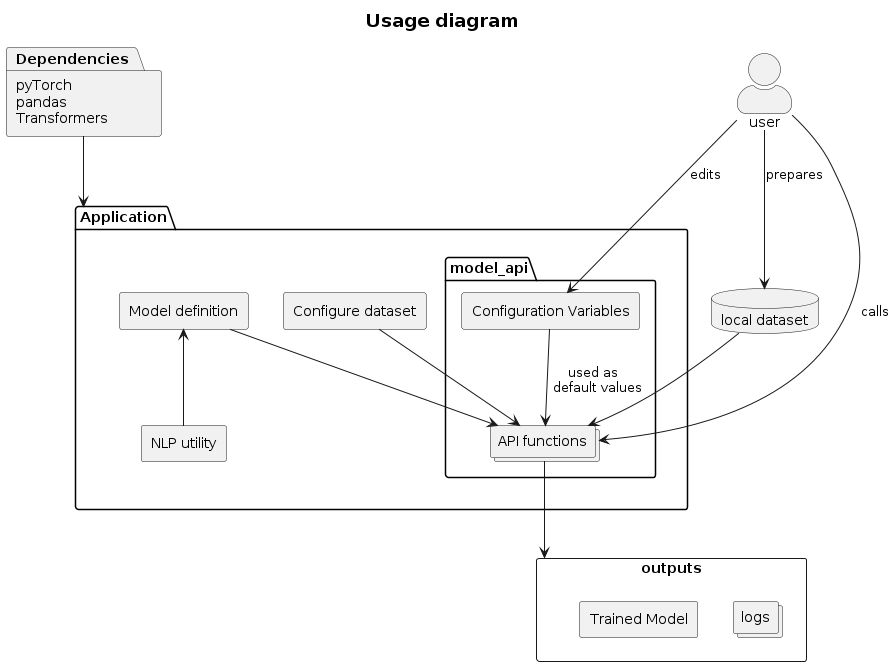
\includegraphics[width=0.99\textwidth]{usage.png}
        \caption{Application usage diagram from the point of view of a user.}
        \label{fig:usage}
    \end{figure}

   We now present our explicitly coded steps for the application execution. The main classes and steps for the processing will be shown here.  For a more detailed view or for all the explicit code, please refer to the documentation handed it together with this report. Please note that \textbf{the functions showed here are not the whole implementation}, some private\footnote{Python does not have private methods and attributes per se, but they can be signalled with a leading underscore ``\_''. These kind of implementation details have been left out} methods and properties have been deliberately left out, as they are not relevant to the conceptual functionality. Likewise, convenience functions (functions created to make the code more readable, boilerplate functions and the like) will be omitted from this overview to avoid bloating.

   \section{Original Code - Dependencies}
   The dependencies needed are Pandas, Seaborn, Matplotlib, \textit{PyTorch} and Transformers.

   All libraries are available through the \textbf{Python Package Installer} (PyPI). The user does not need to install dependencies explicitly. Assuming the user will install this application, the dependencies will be taken care of automatically by the installation process, .e.g.

   \begin{lstlisting}[language=bash]
   pip install -e path_to_the_package
   \end{lstlisting}

   The package will not find its inner dependencies if it is not properly installed, so this step is necessary for the implementation to work.

    \section{Original Code - Reporting and Logging}
   An application generating reports that are easily accessible, easily readable and if possible, easy to parse programmatically is a small step that can greatly enhance the development of a project.

   With this in mind, we have also implemented a system of logging throughout the application, in order to assess its progress and help understand the process executed, especially when in search of bugs and logical errors.

   Both the reporting on the execution content and the logging on the execution progress have routed through the same implementation. It leverages the standard Python \textbf{logging module}. For this purpose we exploit the hierarchical nature of the logger objects of the Python standard library\footnote{\url{https://docs.python.org/3/library/logging.html}}. Throughout the application we send messages to two different loggers, ``printer'' and ``TFM''. They will gather the messages sent to them, and send them up the logger object hierarchy.

   In the API implementation we implemented a method that attaches specially designed handler objects to the main top-level logger (root logger). Those handlers are made to organize and process the logged messages throughout the application according to their level of severity and origin.
   \begin{itemize}
       \item Anything logged in the logger ``printer'', will printed on-screen, as a message from the standard ``print'' command.
       \item Anything logged to the ``TFM'' will be printed on screen only if their severity level is ``Warning'' or above, with contextual information of where it was logged, and its color-coded level of severity (see Fig.~\ref{fig:log_on_screen}).
       \item Anything logged to any logger (``printer'', ``logger'' or any user-created logger) will be printed in two different files:
       \begin{itemize}
           \item A text file that will receive all logs with contextual information, and write in on the file as a normal message (human-readable).
           \item A text file formatted in ``jsonl'' format, in which each of lines printed corresponds to one log, and it is printed in structured json format. The purpose of this file is to provide an easy way to programmatically parse logs and get information out of them, if the user so desires.
       \end{itemize}
   \end{itemize}.

   \begin{figure}[ht!]
        \centering
        \includegraphics[width=0.75\linewidth]{log_message.png}\\
        \includegraphics[width=0.50\linewidth]{logerror_screen.png}
        \caption[A screenshot of on-screen log messages]{Log messages on-screen. Warning on top, Error on bottom. Both with contextual information and color coded to its level of severity}
        \label{fig:log_on_screen}
   \end{figure}
   With this approach in place we can easily get information of our application which helps us understand the process being executed.


   \section{Original Code - Pre-processing of the data}\label{Implementation: Data preprocessing}
   From the user point of view, all that is needed is a pandas DataFrame. Its columns should be labelled the application refers to the data by column labels.  If this is not the case the program will simply crash later when labels are needed, with an explanatory error message about missing labels. Obviously it needs to hold in it the information that we want the NN to learn, i.e. at least two columns to establish a relationship between them.

   \subsection{The CategoricDataset class}
   Once we have the DataFrame with the data, it can get to the first layer of our implementation: \textit{The CategoricDataset class}. It is defined inside the file \textbf{dataset\_define.py}.

   The \textit{CategoricDataset} class is simply a wrapper around the pandas DataFrame, which will execute some steps to organize and label the data for use in the application down the line. It also inherits from \textit{TorchDataset}, as intended by the \textit{PyTorch} Documentation~\cite{pytorch_usermanual}. Even though no functionality from it is used explicitly, it is needed by some automatic processes of \textit{PyTorch} under the hood, over which we have no visibility or control. Hence this inheritance is necessary.

\begin{tcolorbox}[title=CategoricDataset class - From the docs]
    A custom dataset class for handling categoric data.\vspace{5mm}

    This class is used to prepare the data for training the neural network.
    It is designed to work with datasets that have labelled columns.

    The class provides methods for defining the input and output columns,
    splitting the dataset into training and testing sets, and balancing the dataset.

    The class also provides methods for grouping the data by the input columns
    and aggregating the outputs, and for standarizing the data.

    The class inherits from the TorchDataset class, which is used by the DataLoader

    \begin{itemize}
    \item Methods:
        \begin{itemize}
            \item define\_input\_output: Defines the input and output columns to be used by the dataset.
            \item train\_test\_split: Split the dataset into training and testing sets.
            \item cherry\_pick\_split: Cherry pick a row from the training set and add it to the testing set.
            \item balance: Balance the dataset by duplicating rows to come closer to the mean count.
            \item standarize: Standarize the dataset by normalizing the data.
            \item group\_by: Group the data by the specified input columns and aggregate the outputs.
            \item \_\_getitem\_\_: Returns the item at the given index.
        \end{itemize}

    \item Attributes:
        \begin{itemize}
            \item data: The data to be used by the dataset.
            \item input\_columns: The names of the columns to be used as input.
            \item output\_columns: The name of the column to be used as output.
            \item category\_mappings: A dictionary mapping the input and output categories to unique identifiers.
            \item \_already\_configured: Whether the dataset has already been configured.
        \end{itemize}
    \end{itemize}
 \end{tcolorbox}
   \subsection{Functionality breakdown}\label{Section: Methodology_dataset}
   \paragraph{define\_input\_output}
   The first function to be run any time the application starts. This function is in charge of 2 crucial steps. One is to define which column will be an input and which one will be the output, identified by labels.

   Next, it iterates over all the possible values in the input or the output and assigns them unique numeric identifiers. This identifier will be necessary during training and during output identification. All those values are stored in a dictionary called \textbf{category\_mappings}. This dictionary will be used under the hood by the NN model to identify categories, both during training and during execution of a trained model.

   \paragraph{train\_test\_split} Utility function to split a part of the data and return two separate instances of \textit{CategoricDataset} with a desired proportion (e.g. 80\% to 20\% training-validation ratio).

   For flexibility and for ease of use during testing, this function also offers some built-in functionality to deal with some extreme cases:

   \begin{itemize}
        \item Train with all data: If the requested training proportion is 100\%, the testing set will also be set to 100\%. Whether this makes sense is debatable, but it was set up to explore implementation behaviors.
        \item Output presence in training: The method also checks if there are values of the output present in the testing set that are not present in the training set. If so, it tries to solve it by cherry picking rows.

        \item cherry picking rows: To avoid having unseen outputs in the testing set, a cherry picking splitting procedure was implemented. It works by mostly taking out random rows to be put in the testing set, but blocking it if their presence count in the training set would become too small. To be accepted as part of the testing set, it needs to have a presence count in the training set greater than 1 and greater than the mean of all category counts minus 3 times its standard deviation. This gives us still an acceptable random testing set, unless our input data is unbalanced to the extreme. If that were the case, there is not much we can do in the current implementation. We are just stuck with bad data.
    \end{itemize}

    \paragraph{balance:} If the training set is unbalanced (i.e. there are some very evidently underrepresented classes), this function attempts to mitigate it. It simply duplicates entries of the minority class to bring their presence count up (plain Oversampling). It achieves that by copying entries whose count is below the mean by a margin greater than 3 times the standard deviation. It copies it until its count is brought within 3 standard deviations of the mean\footnote{Obviously after that, the mean and the standard deviation will change. But by then this method is done.}
    This is meant to make the minority classes more relevant in the training.
    \begin{tcolorbox}[title=Rework candidate: Approach to data unbalance , colback=white,colframe=blue!50!black]
    This approach of cherry picking rows is very flawed, but it is simple to implement and test, and for a moderate amount of unbalance works pretty well. However, in the datasets we used when attempting practical implementation in Section~\ref{Implement: Practical}, this could easily get out of hand with the dataset sizes, causing the model to overfit a lot by training on oversampled data. A careful measure of how much oversampling is done is necessary, and it is unfortunately very dataset-specific. Hence, a reworking of this feature would be a priority in sustained development.
        \begin{tcolorbox}[title=Future Development: A better handling of unbalanced datasets, colback=white,colframe=green!40!black]
        Finding a better way to mitigate the unbalance of data in the input dataset.
        \end{tcolorbox}
    \end{tcolorbox}


    \paragraph{standarize} Simple function to standarize the data. In the implementation it turns all strings lowercase.
    \begin{tcolorbox}[title=Future Development: Different kinds of standarization, colback=white,colframe=green!40!black]
         If other types of data or different standarization modes would be desired, this would be the place to add it. This could include normalization of inputs, or any other pre-processing step that would be required before having a dataset ready to be used.
    \end{tcolorbox}

    \paragraph{group\_by} Function to aggregate all the inputs. This is done because from the original dataset, a single input can have multiple outputs, but in the DataFrame this means different independent rows. This is ok for training, mostly, but we need to aggregate them when checking. Otherwise we are going to miscount the correct classifications. The joining is straightforward: All entries belonging to the same input are fused into a single entry, and all the different outputs are joined in a list. The list is ensured to hold only unique output elements. If any would be repeated, they are considered redundant and eliminated, as it would just complicate the procedure if the same target output is accounted several times for the same input.

    \paragraph{\_\_getitem\_\_} Crucial method for implementation around \textit{PyTorch}. In standard python \textit{\_\_getitem\_\_} is a \textit{magic method} enabling a class to return a value when accessed via index notation. This functionality is exploited by the \textbf{\textit{pyTorch DataLoaders}} to perform \textbf{data batching} and therefore \textbf{we must implement it}. This implementation will also condition how we process the batched data down the line. In this case, we kept the method as simple as possible. For a given index we return two elements: a list of strings with the values of each of the input columns, and a list of strings of each of the values of the outputs, i.e, each of the returned lists has exactly as many elements as there are features. Note that if there is a single input feature and a single output feature, they still return as lists with a single element, to simplify their handling later.

    Also, if the dataset has executed the \textit{group\_by} function, several outputs might have been aggregated. This is handled by returning the string representation of the list. This means that what we return is not an actual list, but still a string, and if we want to extract the the individual outputs of a given feature, we will have to process it ad hoc.

    \subsection{Summary}
    With this section, we have given an overview of how the data is processed into usable formats for the model. In a real implementation scenario most of this steps will be hidden from the user, as they are easily handled by the API at a higher level.

   \section{Original Code - Implementation of the Neural Network}\label{Implementation: NN}
   The Neural Network (NN) implementation is the core of this application. It is implemented in the file \textit{learning\_model.py}. It is a single class named \textbf{CategoricNeuralNetwork}.

   It leverages the functionality of \textit{PyTorch} to flexibly and easily build a NN according to given high-level specifications, and it also holds all utility functions that the API (or a direct user) will need to run the application. It inherits from \textit{torch.nn.Module}, which allows delegating a significant amount of functionality to \textit{pyTorch}. This includes accounting for parameters to be trained and account for them in gradient calculations. These are hidden from our implementation, in true blackbox fashion.

   \begin{tcolorbox}[title=CategoricNeuralNetwork - From the docs]
    A neural network model for categoric data. The model can be trained using a dataset containing input and target output data. The model
    can be trained to predict the output data based on the input data.

    The model is designed to work with categoric data..
    It can be used to predict categories based on the input data.

    The model can use embeddings for the input and output data. The input data can be
    embedded using a pretrained NLP model, and the output data can be embedded using
    the same model. Each embedding is applied independently of each other.

    The model can be trained to update the embeddings of the NLP model. This can be
    useful when the model is used in a domain-specific context where the pretrained
    embeddings are not sufficient.

    The model can be configured to use a different number of hidden layers and neurons
    in the hidden layers. The number of hidden layers and neurons can be specified when
    creating the model.

    \begin{itemize}
    \item Methods:
        \begin{itemize}
            \item add\_layer: Adds a layer to the model.
            \item build\_neural\_network: Builds the neural network.
            \item forward: The forward pass of the model.
            \item train\_loop: The training loop of the model.
            \item test\_loop: The testing loop of the model.
            \item evaluate: Evaluates the model on a test instance (direct).
            \item execute: Executes the model on a test instance (wrapper of evaluate).
        \end{itemize}

    \item Attributes:
    Besides the variables for flag storage and configuration (given from the argument in the instance creation call), we have:
        \begin{itemize}
            \item \_config: Holds arguments used on instance creation, for easy access and reproducibility. They are also needed for  saving and loading the model from the API point of view.
            \item relu\_stack: The neural network model.
        \end{itemize}
    \end{itemize}
   \end{tcolorbox}

    \subsection{Functionality Breakdown}
    \textit{CategoricNeuralNetwork} is very extensive and implements a lot of different steps and logic. Therefore we shall break it into smaller sections for clarity

    \subsection{CategoricNeuralNetwork - configuration step}
    Given the arguments to the \textit{\_\_init\_\_} method, the class will undertake an extensive configuration process. It will:
    \begin{itemize}
        \item Initialize the object in charge for NLP embedding (instance of \textit{NlpEmbedding}).
        \item Create the Neural Network with the \textit{build\_neural\_network} method.
        \item Initialize the weights of the NN parameters.
        \item Store a \textit{dictionary} called ``config'' that keeps the arguments used by the \textit{\_\_init\_\_} method. Those variables will be necessary for the API to re-create the object when loading it from memory, and hence storing them in an dictionary is an easy way to handle them (reading, copying, accessing and serializing).
    \end{itemize}

    \subsection{CategoricNeuralNetwork - Building the neural network}\label{Section: Methodology_NN_init}
    \paragraph{relu\_stack:} is an instance of \textit{PyTorch}'s \textit{torch.nn.Module}, holding the architecture of the model. It behaves like an iterable, where each of its elements is another instance of \textit{torch.nn.Module}. Each of these instances, represents a layer of the NN. Hence, this is the core of our model, and other functions are dedicated to building it, modifying it, or executing it. A \textbf{forward pass through our model, will necessarily mean a forward pass through the \textit{relu\_stack} object}, which in turn means a forward pass through each of its elements.

    \paragraph{add\_layer:} Method that adds a layer to the relu\_stack object. It is used to build the architecutre of the NN modularily. It takes the type of layer to be added as argument and the number of neurons, and can also automatically add utilities like activation and dropout and Batch normalization layers after it. Its purpose is to facilitate building different NN with some simple high-level commands.

    \begin{tcolorbox}[title=Failed Approach: Using RNN layer , colback=white,colframe=red!60!black]
    Currently, the only accepted type of layer to be added (besides the utility layers mentioned) is linear. It was attempted to use an Recurrent Neural Network (RNN) layer. It was expected that an RNN layer could be beneficial to the performance, because they are very successful and processing NLP tasks.

    However, implementing an RNN failed to produce better results. This is attributed to the fact that RNN layers are good at processing NLP tasks \textbf{when the context is important.} As shown in Section~\ref{Theory: NN}, RNN layers have a mechanism to persistently store information of previous passes (which can be interpreted as context). In our case, this makes no sense, as each of our inputs is, in fact, independent of each other. Ultimately this means that there is no meaning on trying to hold on to contextual information, i.e. the entries that came before. Even worse, having entries that came before affect the learning of the processed input, means that the order in which we would check inputs is relevant, and this \textbf{does not apply to our case}. On top of that, the implementation is very unhandy with our current structure, so it was removed from the code entirely, for the sake of clarity. Why RNN are inconvenient to implement in our current code structure is explained on Appendix~\ref{Apx: A note on implementing RNN}
    \end{tcolorbox}
    \begin{tcolorbox}[title=Future Development: More flexibility when adding layers, colback=white, colframe=green!40!black]
         As of now, the layers added are always in the same order: Linear layer - Batch Normalization - Activation - Dropout. The order is relevant, and it makes sense to have the dropout be the last, because we just want to block some outputs from reaching the next layer, so doing it as a last step ensures that. However, whether we should Normalize before activation is not so clear. No literature has been found regarding this aspect, and in fact both approaches seem to have been used. We placed Normalization first simply because it is how it was used in the paper that introduced them~\cite{ioffe2015batch} (Ioffe, 2015), and it seemed to produce better training results with our particular datasets. This assessment can be an interesting subject of deeper development with broader testing in the future.
    \end{tcolorbox}

   \paragraph{build\_neural\_network:} Automatically builds the the neural network by calling \textit{add\_layer} repeatedly with parameters defined ad-hoc from the configuration variables. There are several logical steps involved:
   \begin{itemize}
       \item Assess the size of the input: The size of the input will necessarily be the number of neurons in the first layer (input layer).
       \item Assess the size of the output: The size of the output will necessarily be the number of neurons in the last layer (output layer). See additional considerations on sizes on Appendix~\ref{Apx: input and output sizes}.
       \item Add input layer: Adds the input layer according to specifications using the \textit{add\_layer} method.
       \item Add hidden layers: It will add as many hidden layers as requested by the configuration variable repeatedly calling the \textit{add\_layer} method. Additionally, it will generate a progression of how many neurons there should be in each layer. The rule of thumb is that it will gradually decrease from the size of the input to the size of the output.
       \item Add output layer: Add last layer according to specifications using the \textit{add\_layer} method.
   \end{itemize}
   The process will always add all three utility layer types after each added layer, except on the output layer, whose output is directly taken as the output of the NN.

    \subsection{CategoricNeuralNetwork - Defining a forward pass}

    \paragraph{forward:} Method that is required by instances of \textit{torch.nn.Module}. This is automatically called whenever a forward pass is executed. Many steps require it, besides the obvious explicit call for the model execution.

    Since our inputs are strings,\textbf{ we need to preprocess them} into an expression that fits our network. This is their embedded representation, with the corresponding model if using embeddings, or a one-hot encoded vector, in case we are simply using categoric ids. Once the representation is computed, the data is given to the relu\_stack, to execute its forward pass, and its outputs are returned. \textbf{The outputs of a forward pass through the NN are called logits}. The logits need to be postprocessed to become understandable inputs, for example identifying the relevant outputs from their value (by index, or cosine similarity. see Apppendix~\ref{Apx: A note on the loss functions} for more detailed explanation).

    \subsection{CategoricNeuralNetwork - The training and test loops}
    \textbf{The train and test loops are the core of the training process}. Both take a \textit{DataLoader} as argument and  a loss function which needs to be an instance from corresponding class in the \textit{PyTorch} library.

    The DataLoader produces batches of data (sets of inputs and their corresponding outputs) from the dataset from which it was created. The batches have a size specified by a parameter when creating the \textit{DataLoader}.

    Both methods then execute a forward pass through the model with the given data batch. Then apply the loss function to the results of the forward pass, and it assesses the correctness of the output against the given targets.  All of this is delegated to the methods inside the loss function instance.

    Note that both train and test loops can (and should) be receiving different batches of data during a training process. \textit{train\_loop} should be getting batches emitted by the DataLoader associated with the training set, while \textit{test\_loop} should be receiving them from the testing dataset.

    Generally, the procedure is to run a training loop on the entirety of the train dataset, and then run a test loop on the entirety of the validation dataset. This 2-step process is one iteration of the training process that we call an \textbf{Epoch}.

    \paragraph{train\_loop:} Besides the loss function argument, the train\_loop also takes an optimizer object as argument, which also needs to be an instance of the corresponding class from the \textit{PyTorch} library. Once the loss has been computed against the expected targets we can proceed to update the model. First all gradients are set to 0. Then the ``backward'' method of the loss function can be executed to make \textit{PyTorch} compute the gradients backpropagation~\cite{Rumelhart1986_Backpropagation}. Lastly, the optimizer can apply the change to the parameters' values based on them using its ``step'' method. \textbf{That is the exact point in which the NN will change to adapt to the targets. The  key lines are shown in Lst.~\ref{Listing: core training}}.

    \begin{minipage}{\linewidth}
    \begin{lstlisting}[language=Python, title=From the implementation of train\_loop method: Core of the training step, caption= Key function calls in the training step that compute and apply the changes to be done to the NN parameters. (with some comments added for clarity),label=Listing: core training ]
    # forward pass
    batch_logits: torch.Tensor = self(x)
    # compute loss of the whole given batch
    loss: torch.Tensor = self._get_batch_loss(loss_fn, batch_logits, y)
    # Backpropagation - ORDER MATTERS!:
    # Set all gradients to zero
    optimizer.zero_grad()
    # Compute the gradient using backpropagation
    loss.backward()
    # Execute changes to the model
    optimizer.step()
    \end{lstlisting}
    \end{minipage}

    The method also has a built-in check in case that, for any reason, the parameters are no longer being updated. This could happen if the learning rate has been scaled to be too small, or if there is some error on the configuration. Unlike with the loss functions, there is no check in-place for the type of Optimizer selected, and any instance coming from \textit{PyTorch} will be accepted. The one found to work the best experimentally in our case is \textbf{AdamW} (detailed explanation on AdamW optimizer found in Section~\ref{Theory: Optimizers}).

    \paragraph{test\_loop:} Computes the loss against expected targets. Once this is done, it proceeds to check the correctness of the results against the target outputs. That is, for the whole dataset emitted by the \textit{DataLoader}, it counts the number of correct guesses, wrong guesses, and guesses that should have been made, but weren't. To do that, it needs to process the logits into the categorization that they represent. This is easier said than done. It is still quite straightforward if the output is categorical as a hot-encoded vector but if the outputs are to be understood as vectors in the embedded space, some post-processing is needed. In particular, we need to measure the similarity of the produced outputs against each one of the possible outputs in the embedded space. We have to do that using the cosine similarity between vectors. This calculation produces a number, and we need to make an arbitrary decision on which is the threshold of similarity, after which we consider a possible output as ``relevant'' or ``chosen''.  See a more detailed explanation on the counting logic in Appendix~\ref{Apx: A note on counting metrics}.

    When the whole given dataset has been accounted for, we can compute the \textbf{F1 Score, the Precision and the Recall of our model}(metrics presented in Section~\ref{Theory: NN-considerations}). Those metrics are then returned, so they can be used to evaluate the progress and decide whether to stop training.

    \begin{tcolorbox}[title=Rework candidate: Approach to cosine similarity , colback=white,colframe=blue!50!black]
    We decide whether an possible output is relevant by checking if the logits cosine similarity with it is over a threshold. But it is not clear which is a good threshold of similarity to consider a possibility as relevant, an iterative approach was taken. Considering the cosine similarity result for each of the outputs, the metrics F1, Precision and Recall are computed considering different thresholds for relevance of the cosine similarity. Then, the threshold that produces the best F1 value is picked. The value is saved in the model, and becomes the cosine similarity threshold to use, until (and if) it changes again in another \textit{test\_loop} execution. If this is the last loop, then the value will remain saved in the model as an attribute for when an evaluation is run with the trained model.
        \begin{tcolorbox}[title=Future Development: Find a better way to handle cosine similarity thresholds, colback=white, colframe=green!40!black]
        Optimizing and finding a more robust way to choose a threshold, without having to do trial-and-error with different values to choose the best ad-hoc.
        \end{tcolorbox}
    \end{tcolorbox}
    \begin{tcolorbox}[title=Failed Approach: Train all labels in multi-labelled input at once, colback=white,colframe=red!60!black]
    In the way that it is implemented right now, the training dataset is not aggregated. This means that if an input has more than one output, rather than appearing once with all the labels in the dataset, it appears once for each label, as independent entries. This works, but seems inefficient.

    It was attempted to aggregate the inputs before training, in order to have the loss function assess the loss against all targets that are relevant for the input at once. Theoretically, one would expect to be significantly more efficient. The reasoning of why can be found in Appendix~\ref{Apx: A note on aggregating multilabeled inputs}. This approach was implemented, but failed to produced good results, and it was discarded. Still seems it should be a robust approach to training.
        \begin{tcolorbox}[title=Future Development: Find a way to train multi-labelled inputs in one single forward pass, colback=white, colframe=green!40!black]
        As stated, it seems logical that training multi-labelled inputs at once with a single forward pass should be massively more efficient, both because of reduced number of entries per epoch, and because we could avoid conflicting training. Considering this, it seems likely that the reason why this implementation failed did not lay with the idea itself, but rather the execution, but there was no more time to experiment further. Therefore, this is left as an option for future development.
        \end{tcolorbox}
    \end{tcolorbox}
    \subsection{CategoricNeuralNetwork - Evaluating the model}\label{Section: Methodology_NN_exec}

    \paragraph{evaluate:} Method to explicitly run forward pass. It has some low level handling, so the input and the output at properly handled in terms of syntax i.e. ensure the dimensions are correct, that the inputs are the correct type... It can be understood as a low-level wrapper around the forward method.

    \paragraph{execute:} Method that acts as a high level wrapper for the evaluate method.  The execute method takes care of higher level handling of inputs and outputs. That means that a call to execute will take any format for the input, i.e. a string, a list of strings, a list of lists... and properly handle it. It will also take care to post-process the outputs into the correct category. In other words, ``execute'' makes the whole process of getting readable outputs from the model completely seamless and blackbox-like. A user should run the execute method rather than the evaluate to take advantage of this higher level assets.\textbf{ The method has 3 operating modes}:

    \begin{itemize}
        \item Monolabel: Returns the single best match to the logits. (single label classification).
        \item Multilabel: Returns all the matches to the logits, as their probability associated to the label is over a set threshold.
        \item Priority: Return all possible output labels, but ordered in decreasing order of relevance.
    \end{itemize}

    \paragraph{add\_output\_category:} Method that adds a possible output value to an output feature. It needs the output feature name and the value to be added. Then it will add it to the dictionary \textit{category\_mappings.} This does nothing for the training process, but once the NN has been trained, it can be useful to add a new field without having to retrain the NN from scratch. Ultimately this is reasonable because if the outputs are embedded, the size of the output layer is fixed by the embedding dimension, so it will not change if new outputs are added. Furthermore, the choice of output labels works by comparing them with Cosine Similarity. So A well trained NN should be able to handle them on the fly without additional training.

    Note that adding a new output label would make a model that does NOT use output embeddings obsolete. In that case the output is a multi-hot vector of dimension equal to the number of output possibilities. Hence, adding one would mean that the output size needs to increase by one, and this is an architectural change. Therefore, if output embeddings are not being used, this method will throw an error and halt the program.

    \subsection{CategoricNeuralNetwork - Summary}
    With this section we have presented the central module of our implementation, the NN itself. We have covered the most important methods and logical steps to understand what it is does at a conceptual level, and we touched upon its connections with the other modules: The \textit{PyTorch DataLoaders} as a link to the training and validation data, and the calls to the NLP utility to produce embeddings, which we will be presenting in the next section. See a diagram of those relationships in Fig.~\ref{fig: Flow}.
    We have also shown the flexibility and dynamism of the class given its parameters, and we laid the ground work for the later presentation of the API.
   \begin{figure}[ht!]
       \centering
       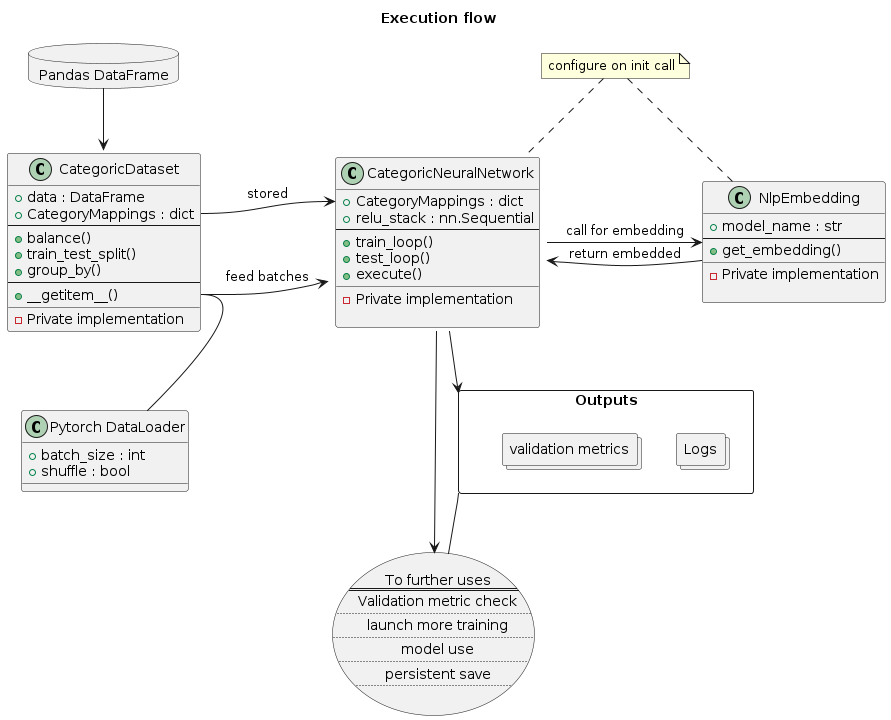
\includegraphics[width=0.75\linewidth]{flow.png}
       \caption[Flow of the core application]{Class hierarchy and calls showing the flow of execution in the application around the Neural Network model. The connecting links are handled by the API}
       \label{fig: Flow}
   \end{figure}

   \section{Original Code - Implementation of the Natural Language Processing Layer}\label{Implementation: NLP}
   The NLP layer has been completely detached from the implementation of the model. It is found in the file \textit{nlp\_embedding.py}.

   The main object is the class \textbf{NlpEmbedding}, which is a very compact simple class whose only purpose is to hold the embedding model and return the embedded expression from given inputs. In the structure of the project, the class \textit{CategoricNeuralNetwork} initializes an instance with the given specifications (the embedding model name), and keep the instance as an attribute for its internal use.

   \textbf{The class \textit{NlpEmbedding} initializes the tokenizer and embedding model based off the library Transformers}~\cite{huggingface_transformers}. Transformers offers a huge array of pre-trained models, and they can simply be chosen by name. In the current implementation, the name is a given argument to the initialization call of the \textit{NlpEmbedding} class. If the model is available, it will initialize it and store it as an attribute, and if it is not, it will attempt downloading it so it can be likewise used (this is is included in the Transformers automatically provided functionality under the hood). The class wil likewise initialize the corresponding model tokenizer.

   \begin{tcolorbox}[title=NlpEmbedding - From the docs]
    Class to handle the NLP embeddings.

    \begin{itemize}
        \item Args:
        \begin{itemize}
            \item model\_name: The name of the model to be used for embeddings.
        \end{itemize}
        \item Attributes:
        \begin{itemize}
            \item tokenizer: The tokenizer used for tokenizing the input data.
            \item embedding\_model: The model used for embeddings.
        \end{itemize}
        \item Methods:
        \begin{itemize}
            \item get\_embedding: Gets the embedding for a given text.
        \end{itemize}
    \end{itemize}
    \end{tcolorbox}
   \subsection{Functionality Breakdown}

   \paragraph{Initialization step}: Use \textit{PyTorch}'s native functionality to import the tokenizer and embedding models by name, and save them as attributes.

   \paragraph{get\_embedding}: Method that will take an input and return an embedded output. This is the function that gets actively called from the \textit{CategoricNeuralNetwork} instance.

   The method itself has the minimal logic in place to produce the embeddings, and return them in a tensor of equal dimension. i.e., if given a single piece of data to embed, it will return a single tensor, if given $n$ entries to embed (an n-sized batch), it will return a tensor of dimension $n$ in which each of the elements corresponds to the embedding of one of the entries.

   In terms of how the embedding is computed, the process is very straightforward once the tokenizer and the embedding model are initialized:

   \begin{itemize}
       \item \textbf{Process the data with the tokenizer:} This produces  a tensor of tokens and a tensor of attention.
       \item \textbf{Embed the tokens with the attention tensor:} Apply the embedding model on each of the tokens produced. The attention tensor will take care to mark the meaningful tokens only, while the padding will get ignored.
       \item \textbf{Pool the embedded tokens in a single embedding for the entry:} Once all tokens have been correspondingly expressed in the embedding space, the combined embedding of all them can be computed by pooling (aggregating them in a single vector in the embedded space). The pooling strategy can be chosen as an argument of the function call. By default we use the mean of all embeddings. \textbf{This produces the final embedding for the processed entry.}
   \end{itemize}
   If the input was single entry, we already have  the embedded expression of it, and it can be returned. If the input was a batch, we have a collection of embeddings, one for each entry. In that case, we stack them vertically, so that we are left with a tensor of dimension equal to the size of the incoming batch, and we return it.

    \subsection{Summary}
    Thanks to the \textit{Transformers} library, the implementation of the NLP layer is very compact and straightforward. The implementation is robust and works easily, but further considerations are necessary besides the formal code implementation.

    The most important decision, is which embedding model to use. In our implementation we mostly used 2 different ones depending on the task:
    \begin{itemize}
        \item \textbf{CodeBERTa-small-v1}: It was found to work the best with experimental data.
        \item \textbf{distilbert-base-uncased}: Works poorly on the experimental data, but very well with the implementation used for proof of concept.
    \end{itemize}

    A reasoning for the choice of each of those can be found in Appendix~\ref{Apx: A note on the choice of NLP pretrained models}

    \begin{tcolorbox}[title=Failed Approach have the embedding as part of the NN model, colback=white, colframe=red!60!black]
    Generally, an embedding can be trained to learn to identify semantic meanings that are relevant to the problem itself. In practical terms this simply means to train the weights of the embedding model such that words that are semantically similar will have a close representation in the embedded space.

    As such, it was attempted to have the embedding be part of the training, but this failed to produce any results. The embedding just lost its way completely, failing to find any relationships at all. This was attributed to the embedding model being very big, and that messing with its weights with such a small amount of data as in our models just interfered with it. Perhaps a very small learning rate would have solved that, but the efficiency of running the model fixed with its pre-trained values was already acceptable. So for simplicity, the embedding model was deliberately left as an external piece to our NN model, which simply provided the embeddings on request. This is also the reason why the class \textit{NlpEmbedding} does not inherit from \textit{torch.nn.Module} as this would account for its parameters in the \textit{PyTorch} algorithms.
    \end{tcolorbox}

    \begin{tcolorbox}[title=Future Development: Use a locally trained embedding, colback=white,colframe=green!40!black]
        The embeddings currently used are completely external to the NN and are not specifically trained to the task. While they serve their purpose well, they also imply quite some overhead due to their size. For the kind of problem we are attempting to solve, a much smaller embedding would probably also work fine, especially if it would have a more restricted vocabulary that was relevant for the problem. For that, \textbf{implementing an ad-hoc Byte Pair Encoding} tokenizer that recognize the important patterns as tokens, and \textbf{an embedding that would be trained together with NN} would be a good approach. This would probably make it faster as well. However it would also lead to the need of periodic retraining the embedding and making a new tokenizer (if new keywords or patterns would be added to the data).
    \end{tcolorbox}

   \section{Original Code - Implementation of the API}
   The API is designed to be a wrapper around all the application presented until now. Ideally, a user will only need to interact with the API to do any tasks to run the application. It should be completely straightforward and unchallenging to set up some configuration, and create a model for learning some given data. This has been the target in all steps of the API design.

   The API is stored in the file \textit{model\_api.py}. It is centered around a single class called \textbf{ModelApi}, whose purpose is to be instantiated by the user. The class holds the configuration in an instanced object, and it offers a selection of methods to simply apply the modules we have presented until now.
   ConfigRun is meant to be a class whose only purpose is to store values to which the API can refer during its execution. An instance of it will be created and stored in the API instance, and the user can alter its parameters by direct assignment.

   The configuration object which will be instantiated inside the \textit{ModelApi} class:
   \begin{tcolorbox}[title=ConfigRun - From the Docs]
    A dataclass to store the default configuration for the model training.

    \begin{itemize}
        \item Attributes:
        \begin{itemize}
            \item balance\_training\_data: Whether to balance the training data.
            \item aggregate\_outputs: Whether to aggregate the outputs.
            \item max\_hidden\_neurons: The maximum number of hidden neurons in the model.
            \item hidden\_layers: The number of hidden layers in the model.
            \item model\_uses\_input\_embedding: Whether the model uses input embedding.
            \item model\_uses\_output\_embedding: Whether the model uses output embedding.
            \item model\_trains\_nlp\_embedding: Whether the model trains the NLP embedding.
            \item learning\_rate: The learning rate for the model.
            \item batch\_size: The batch size for the model.
            \item epochs: The number of epochs for the model.
            \item train\_size: The proportion of the dataset to be used for training.
            \item train\_targets: The targets for the training.
            \item optimizer\_name: The name of the optimizer to be used.
            \item nlp\_model\_name: The name of the NLP model to be used.
            \item lr\_decay\_factor: The factor by which the learning rate will be decayed.
            \item scheduler\_type: The type of the scheduler.
            \item scheduler\_plateau\_mode: The mode for the scheduler.
            \item lr\_decay\_patience: The patience for the scheduler.
            \item lr\_decay\_target: The target for the learning rate decay.
            \item lr\_decay\_step: The steps for the scheduler.
            \item out\_dir: The directory to save the reports and outputs.
            \item case\_name: The name of the case.
            \item report\_dir: The directory to save the reports.
            \item report\_filename: The name of the report file.
        \end{itemize}
    \end{itemize}
    \end{tcolorbox}

    \begin{tcolorbox}[title=ModelApi - From the Docs]
    A class to store the functions for creating, training and configuring a categoric neural network model.

    \begin{itemize}
        \item Attributes:
        \begin{itemize}
            \item config: Store configuration variables (Instance of ConfigRun)
        \end{itemize}
        \item Methods:
        \begin{itemize}
            \item configure\_default\_loggers: Configure the default loggers for the module.
            \item wipe\_handlers: Wipe the loggers from the root logger.
            \item reconfigure\_loggers: Reconfigure the loggers.
            \item configure\_dataset: Configure the dataset for training the model.
            \item get\_dataloaders: Get the dataLoaders for the training and testing of the model.
            \item create\_model: Create the model according to specifications
            \item get\_optimizer: Get an optimizer instance.
            \item get\_scheduler: Get a scheduler instance.
            \item get\_loss\_fn: Get a loss function instance.
            \item train: train a model with the given data.
            \item build\_and\_train\_model: Automatically execute everything to produce a trained model from scratch.
            \item save\_model: Save the model and configuration to disk
            \item load\_model: Load the model and its configuration from disk.

        \end{itemize}
    \end{itemize}
    \end{tcolorbox}
   \subsection{Functionality Breakdown:}
   The API itself has very little logic in comparison to previous modules, but still we will break it down into a few sections for structural clarity.
   \subsection{API - Preparation step}
   This should be the first functions that a user executes of the API. The first step is creating an instance of the \textbf{ModelApi} class, and from then on use its methods to direct the flow of the application execution. The values to be used when calling methods are stored in the ``config'' variable. They can be overridden with specific arguments in the call in the method call, in any case. This is ill-advised, as it can be difficult to keep track of all used options and can end up producing consistency problems. However, it might sometimes be useful to just explicit arguments when coding, developing or testing.

   \paragraph{config} Attribute which is an instance of the ConfigRun, holding the values to be used as when running other methods.

   \paragraph{configure\_default\_loggers:} Method that will take care of attaching the default Handler objects to the root logger. It will attach one to send all messages sent to the logger called ``printer'' to the terminal. It will attach one to send all messages with a severity level ``Warning'' and above to the screen, with contextual information and color coded according to the level of severity. And lastly will attach two handlers that will send all logged messages to files, one formatting the messages as ``human-readable'' and the other in the form of a structured json.

   \paragraph{wipe\_handlers:} Method that will delete all handlers from the root logger. Useful if the user no longer wants the default handling of logs and would like to use their own.

   \paragraph{reconfigure\_loggers:} Method that will run \textit{wipe\_handlers} and \textit{configure\_default\_loggers}. This is useful if some configuration value changed (like the path to log files) and the user would like to update the handlers.

   \subsection{API - Initialization step}
   \paragraph{configure\_dataset:} Takes a \textit{Pandas DataFrame}, a list of strings that identify input columns and a list of strings that identify output columns. Creates a \textit{CategoricDataset} and runs its configuration method of CategoricDataset, to pre-process the data and prepare it for further use. Then returns it. That way the user does not need to create and configure the \textit{CategoricDataset} themselves.

   \paragraph{get\_dataloaders:} Method to split the data into training and testing set, and create \textit{DataLoader} instances for each of them. Optionally it can try to balance the training data via oversampling. Optionally it can aggregate the outputs of the testing set (Always a good idea). Returns the training, and test \textit{DataLoaders} in a tuple.

   The size of the batch is also specified in this step. This can be an important consideration and it depends on the data being used. A large size will take more entries into account per optimizing step, effectively regularizing the data and having a better average guess of the overall better changes to apply to make the NN more competent. A smaller batch might be better for perceiving finer details in the data, but it could be susceptible to large outliers which might disturb the optimisation step. Choosing a correct size is important, but there is no rule of thumb. In this implementation the default is size 32.

   \paragraph{create\_model:} Method that creates the instance of \textit{CategoricNeuralNetwork}. It will initalize it with the options given, and will return the instance of the model.

   \paragraph{get\_optimizer:} Method that creates an instance of an Optimizer object from \textit{PyTorch} and returns it. It can return an instance of ``SGD'', ``Adam'' or ``AdamW'' (AdamW is recommended). This method has to take the model as argument, as it needs to collect its parameters to register them for the gradient computation. It also needs to be given a learning rate, which will be the default learning rate of all parameters in the model.
    \begin{tcolorbox}[title=Future Development: allow different learning rates, colback=white,colframe=green!40!black]
    As of now, all parameters in the model share the same learning rate. \textit{PyTorch} supports using different learning rates values for different parameters. This could be an interesting improvement on the model. For example, one the presented failed approaches had to do with the pre-trained embedding models being too sensitive to the training. Giving them a custom reduced learning rate could solve that problem.
    \end{tcolorbox}

   \paragraph{get\_scheduler:} Method that returns an instance of a scheduler class from \textit{PyTorch}. A scheduler is a utility implemented in PyTorch that is able to decrease the learning rate during training according to certain rules. This is intended to stabilize the training process, by reducing the size of the steps taken by the optimizer. This should allow for finer approaching to the solution when in the vicinity of the local solution space. There several kinds of scheduler in the \textit{PyTorch} library, but this function supports only 2:
   \begin{itemize}
       \item StepLR: Reduces the learning rate by a factor when a given number of training epochs have elapsed.
       \item ReduceLROnPlateau: Reduces the learning rate by a factor when an arbitrary quantity given as an argument has failed to increase or decrease (configurable) for a given number of calls to the function. It should be called once per epoch.
   \end{itemize}

   \textit{ReduceLROnPlateau} is recommended because it can react autonomously to the training of the model. When \textit{ReduceLROnPlateau} is used, it will reduce the learning rate, multiplying it by ``lr\_decay\_factor'' when the F1 score has failed to increase for a ``patience'' number of epochs.

   \paragraph{get\_loss\_fn:} Method that returns a loss function instance from the \textit{PyTorch} library. Currently it only supports ``BCEWithLogitsLoss'' and ``CosineSimilarityLoss''. They can be chosen either by name as an argument in the function call, or letting the method automatically decide the suitable one according the current values in the config attribute. If it chooses by itself, it will check whether the model will use output embeddings or not. If it is not using output embeddings it will choose ``BCEWithLogitsLoss'', as the output will be categorical in the form of a hot-encoded vector. Otherwise, it will return ``CosineSimilarityLoss'' to compare the logits with the possible outputs in the embedded space. Choosing the wrong one will cause the model training to crash.

   \subsection{API - Execution step}\label{Section: Methodology_Api_train}
   Once the configuration has been set and all the needed objects and classes initalized, the user can proceed to train and store the network.

   \paragraph{train:} Main method that launches the training and validation of the model, and also generates reports on the process. To train the model all the previous instances are needed: the \textit{DataLoaders}, the model instance, the loss function and optimizer, and optionally, the scheduler. The method then launches the training loop, and immediately executes the test loop after. With the values of the metrics returned by the test loop, it can be decided whether to continue the training or to stop and consider the model as trained.

   This method also takes care of running the scheduler instance if needed, and to generate the summary plot in the output directory to assess the process of training. There is an additional check with the scheduler, in which if the learning rate is found to have become too small, it will also interrupt the training, because continuing will be interpreted as meaningless.

   Additionally, a flag allows real-time plotting of the training, if the user so desires. After it is done, it returns the trained model. The user can use the model freely after that.

   \subsection{API - High level handling}

   \paragraph{build\_and\_train\_model:} This is a function that will take care of running all of the above as needed, to condense all execution in a single function call from the point of view of the user. Given a \textit{DataFrame} and a list of names for the input and output columns, the method will pre-process the data, build the model according to configuration, create the loss function, the optimizer and the scheduler and automatically launch the training process. When it is done, it will return the model.

   This is the method that user should run, preferably after setting the desired configuration in the config attribute.

   \paragraph{save\_model:} Method to save the model to disk. In practical terms, the saved data is only the weights of the parameters of the model, as there is no way to save the whole instance of the trained model as it is. Saving the whole model could lead to consistency problems if it would be loaded from another system, and it is also very inefficient. Instead, the parameters that were used to create the model are also saved in a file, as well as the current API configuration. These two sets of parameters can be used to rebuild the model when loading it from memory. The model weights are saved in a file with extension ``.pth'' while the sets of parameters are save in a file with the same name but extension ``.ini''.

   \paragraph{load\_model:} Method that will load a model from memory and return it. It will take a model by name and load it from the specified path. The path needs to be given without suffixes, and the last component should be base name of the files (i.e., trying to load ``model'' will attempt to read the files in the current directory with names ``model.pth'' and ``model.ini''). It needs both the ``.pth'' file for the weights of the model and ``.ini'' files for the configuration parameters. After reading the configuration parameters, the configuration of the API instace gets overwritten with it. Likewise, a model instance is build from the dictionary of parameters specified in the file. This creates a fitting model that has the same structure as the model that was used as argument for the \textit{save\_model} function. Then all the parameters saved in ``.pth'' file can be applied to this created replica of the model, to set their weights to match the result of the training. Hence, we reproduced the trained model we had. Then returns the model for further use.

    \paragraph{add\_output\_possibility:} Method to call the add\_output\_possbility method of a given model. This will add an output field in its dictionary that accounts for possible outputs, making it possible to be considered when running comparison with Cosine Similarity. This should allow a NN to match with outputs it has not seen before during training.

\subsection{API - Summary}
We have shown the main methods of the API, which are ultimately intended to be the only ones exposed to the user. A user is able to run the application according the their needs, and to easily create and train models with different hyperparameters and between different sets of data with minimal handling. From this point onwards, all tests and executions are run through the API calls, including the tests and the practical implementation.

\section{Proof of Concept - Feature Testing: Learning to identify a sentiment} \label{Section: POC}
This section showcases basic implementations meant to test the robustness of the implemented functionality. We should able to proof that the application works as intended and with a minimal involvement on the side of the user. We also want to illustrate the basic usage case for clarity.

\subsection{Learning from reviews and categorizing pre-generated sentences}
 We take a set of sentences, taken from amazon, yelp and imdb reviews, each properly labeled as positive or negative~\cite{Dimitrios2015_sentiment_labelled_sentences}.  An example of the content in the dataset can be viewed in Fig.~\ref{fig: sentiment_csv}, where we can see the data that will be parsed into a \textit{DataFrame}. It is a set of sentences which are followed by a 1 or a 0. A 1 means that the sentence is labelled as positive, and 0 means it is labelled as negative. This can be stored in a DataFrame with two columns.

\begin{figure}[ht!]
    \centering
    \includegraphics[width=0.75\linewidth]{sentiment_csv.png}
    \caption[Example contents of a simple dataset]{Contents of the sentiment dataset in csv format. There are two fields, one is the sentence to be interpreted in the other is the label. 1 means it is a positive sentence, and 0 means it is a negative.}
    \label{fig: sentiment_csv}
\end{figure}

This is used to train a NN with the API we presented. The code to run this is shown in Lst.~\ref{Lst: sentiment_minimal}. In the code we are defining configuration variables by direct assignment, such as the maximum number of hidden neurons per layer (\textit{max\_hidden\_neurons}) or the number of hidden layers (\textit{hidden\_layers}). Then we state that no output embeddings will be used, as this is a binary classification problem in two categories and there is no meaning to be conveyed in the output category names. We choose a an NLP embedding model (\textit{distilbert-base-uncased}). Since we don't need to set up any custom logger we can set them up automatically with the provided API function. Lastly, we read the \textit{DataFrame}, we indicate the input and output columns and we let the api take care of everything else, including pre-processing the data, creating the NN and training it (all contained in the call \textit{build\_and\_train\_model}).

\begin{minipage}{0.95\linewidth}\vspace{5mm}
\begin{lstlisting}[frame=single, language=Python, title=A minimal code, caption=Simple code using the api to train a NN in sentiment recognition. Dataset is assumed to be given through the get\_data() method, label=Lst: sentiment_minimal ]
    api = model_api.ModelApi()
    # override the defaults, although not strictly necessary
    api.config.max_hidden_neurons = 16
    api.config.hidden_layers = 1
    # turn off output embedding, makes no sense in this case
    api.config.model_uses_output_embedding = False
    # override model with a faster one, not strictly necessary
    api.config.nlp_model_name = "distilbert-base-uncased"
    # Define case name for use as file names
    api.config.case_name = "sentiment\_compact\_n16\_l1"
    # configure the loggers to produce the standard reports
    api.configure_default_loggers()
    # Define the input and output columns
    # get the DataFrame with some pertinent function
    df: pd.DataFrame = get_data()
    input_columns = ["text"]
    output_columns = ["label"]
    # Execute the highest level api method
    model = api.build_and_train_model(
        df=df,
        input_columns=input_columns,
        output_columns=output_columns
        )
    api.save_model(model)
\end{lstlisting}
\end{minipage}

With the code shown above, the API will train the NN until either a metrics target or maximum number of epochs is reached. We will be left with a trained model in our namespace and a persistent save to disk, stored for later use.  In Tab.~\ref{Tab: config parameters} we see the whole set of values in the configuration. Most of them are simply the default values, but we can also see those that were defined explicitly in Lst.~\ref{Lst: sentiment_minimal}.

Additionally it produces the logs and reports mentioned above. The logs will be stored in the directory specified by the corresponding configuration variable (\textit{report\_dir\_name}), and they will be written on by the Handler objects attached to the root logger by the method \textit{configure\_default\_loggers}. See screenshots of the log files content in Fig.~\ref{fig: log_screenshots}.

The plot that shows the progress of training in the form of the metrics (F1, Precision and Recall) vs Epoch number is also automatically generated by the API, see Fig.~\ref{fig: autoplot_report}. If there is a target for one of the metrics defined, it will also show it in the form of a horizontal dashed line. If all the metrics with a target go over it (over their respective dashed lines), the training stops and is considered successful. As seen in the figure, the training was very effective, as it managed to go over the target (F1 score $>$ 0.75) in just 4 epochs.


\begin{table}[ht]
\footnotesize
\centering
\begin{tabular}{|p{4cm}|p{4cm}||p{4cm}|p{2.5cm}|}
\hline
\textbf{Epochs} & 15 & \textbf{Learning Rate} & 0.001 \\
\hline
\textbf{max\_hidden\_neurons} & 16 &\textbf{Batch Size} & 32 \\
\hline
\textbf{Hidden Layers }& 1 & \textbf{Train Size }& 0.8 \\
\hline
\textbf{Use Input Embedding} & True & \textbf{Train Targets} & \{'f1': 0.75\} \\
\hline
\textbf{Use Output Embedding} & False & \textbf{Optimizer Name} & AdamW \\
\hline
\textbf{NLP Model Name} & distilbert-base-uncased & \textbf{Trains NLP Embedding} & False \\
\hline
\textbf{LR Decay Factor} & 0.1 & \textbf{Scheduler Type} & None \\
\hline
\textbf{Scheduler Plateau Mode} & max & \textbf{LR Decay Patience} & 10 \\
\hline
\textbf{LR Decay Target} & f1 & \textbf{LR Decay Step} & 10 \\
\hline
\textbf{Case Name} & sentiment\_compact\_n16\_l1 & \textbf{Report Directory Name} & reports \\
\hline
\textbf{Report Filename} & report & \textbf{F1 Target} & 0.75 \\
\hline
\end{tabular}
\caption[Config parameters of small example run]{Settings of the example execution for sentiment detection. Extracted from human-readable logs. This set of configuration values is the result of Lst.~\ref{Lst: sentiment_minimal}. The values not explicitly assigned in the the code are left to their default values.}
\label{Tab: config parameters}
\end{table}

 \begin{figure}[ht!]
     \centering
     \includegraphics[width=0.32\linewidth]{human_readable_log.png}
     \includegraphics[width=0.55\linewidth]{jsonl_report.png}
     \caption[Logs and reports screenshot]{\textbf{Left Panel}: A screenshot of the human-readable log produced from the code in Lst.~\ref{Lst: sentiment_minimal}. It shows the last training epoch and breakdown of the validation step metrics (F1, Precision and Recall).\\ \textbf{Right panel}: A screenshot of the jsonl format log from the same execution, the same messages that appear on the left panel are highlighted with a red square. Lines shown are cut because they can be arbitrarily long.}
     \label{fig: log_screenshots}
 \end{figure}

 \begin{figure}[ht!]
     \centering
     \includegraphics[width=0.5\linewidth]{sentiment_n16_l1.png}\\
     \caption[Plotted report on training]{Automatically generated report plot that shows the progression of the score of each of the metrics (F1, Precision and Recall) during training epochs. The horizontal dashed line is the training target (F1 score=0.75), and the training stops when it is reached. Epochs are counted in integer increments, although the automatic plotting library shows floating point values as labels in the x-axis.}
     \label{fig: autoplot_report}
 \end{figure}

After the training, we immediately tested the model with some sentences that the model has not seen before, neither in training nor validating. They are stored directly in Python list format in the file \textit{sentences.py}. Those are randomly generated by ChatGPT, completely unrelated to the training set. The application reported an accuracy of correct classifications of 187/188 (99.47\%)  when applying the trained model on the unseen, unvalidated sentences. We can even test it ourselves with interactive python to show the API usage and the model ability. See the example manual execution in Python interactive in Fig.~\ref{fig: sentiment_manual}.  We show the importing of api, the loading of a trained model by name (assuming the interpreter is running in the same directory, otherwise a path has to be given), and a direct execution of the model by giving it an input through the function \textit{execute}. The return values of the \textit{execute} method are printed on-screen showing the successful classification of the random sentences entered. We show also how the model can handle a single input (given as a \textit{str}) or several at once (given as a \textit{list[str]}) and correspondingly return the associated outcomes. This is proof that our implementation is robust and functional.

\begin{figure}[ht!]
    \centering
    \includegraphics[width=1.0\linewidth]{sentiment_manual.png}
    \caption[Example running on Python Interactive]{Running the application from Python interactive. It shows basic API commands on-screen and the execution of the model.}
    \label{fig: sentiment_manual}
\end{figure}

\subsection{Summary}
With this simple test example we have shown both the ease of use and the reliability of the implementation. The application was capable of seamlessly creating a NN, train it (with 20\% of the data used for validation only) and effectively learn to identify the overall sentiment of arbitrary sentences with an accuracy of 187/188 correct classifications. We have also shown how we can use the API to import and execute a forward pass of the model, all with an intuitive simple syntax. Therefore, \textbf{we can state that the implementation is robust}.

Both the dataset and codes used are delivered together with the application, for local testing purposes. They can be found with the \textit{test\_codes/} directory in the application module. That way a user can locally test the implementation themselves, before moving on to actually make use of it.

\chapter{Practical Implementation}\label{Implement: Practical}
We have a working and functional implementation and an API that allows us to tailor it and execute according to a configuration ad-hoc. Our objective was to develop an application for automatising test method selection in a repository based on NLP processing of the function names. We are now going to show the practical implementation of this objective, and we will analyze the results.

In the idealized practical implementation, the application would be embedded in a repository. Then it could be taught the relationships between functions and their relevant test methods to achieve an autonomous capacity to choose, or at least prioritise, tests to be run given changes reported or detected. The fundamental idea is that by training the model to associate method and tests through NLP layers, certain benefits could be achieved:

\begin{itemize}
    \item If a change is detected in a function in the repository, mark relevant tests to be run.
    \item If a new function or test method (or both) appear in the repository, make a good guess on the tests that might be relevant based on its name.
    \item Detect possible correlation about tests by name, that could be relevant, even if in the original training dataset it was not explicitly stated (i.e., detect non-obvious correlations).
\end{itemize}

This idealized outcome sets us on track on how to analyze and how to evaluate the success or failure of our implementation.
\section{Dataset used}
Our base is the \textit{methods2test} dataset~\cite{tufano2021unit}. \textit{methods2test} is a supervised dataset consisting of Test Cases and their corresponding Focal Methods from a large set of Java software repositories. In our case we wish to relate the Focal Methods (functions) to the tests that are relevant for them. The information parsed from the dataset can be summarized in 4 columns:
\begin{itemize}
    \item repository\_id: A unique identifier for the repository to which a method belongs.
    \item method\_name: The name of a method.
    \item method\_params: A string with the argument types for the method call.
    \item method\_return: A string with the argument types for the method return.
    \item test\_case\_name: The name of a test method which is relevant for the method \textit{method\_name}
    \item test\_class\_class: The name of the class (a grouping) to which the test method \textit{test\_case\_name} belongs.
\end{itemize}

We could attempt to create a NN to relate any of these fields to any other. What makes sense to us though, is to try to relate the \textit{method\_name} to \textit{test\_case\_name}.

    \begin{tcolorbox}[title=Failed Approach: Using multiple inputs simultaneously , colback=white,colframe=red!60!black]
    It was considered to use simultaneously \textit{method\_name}, \textit{method\_params} and \textit{method\_return} as inputs for the neural network. The implementation supports this kind of multiple-feature input without problem. However this was discarded. It did not produce significantly better results, and complicated the use of trained neural network quite a bit on the user side, when handling input of different features. On top of that, it was considered that while theoretically, the type of arguments or return of a method can be decisive in choosing whether a test is relevant or not, it was unreliable for this kind of task. This is attributed to the types being quite common, i.e., many functions are going to take int, float, char or the like, as input or as return value and not that strong of a pattern can be established. In the very specific cases, like a type being custom class, this could be very useful, but they generally happen too scarcely for a successful training of NN.
    \end{tcolorbox}
Hence, we can parse the entirety of this dataset, and configure a set of smaller datasets for testing purposes. These smaller datasets are stored in csv files, for easy access and are delivered together with the application for testing purposes. They can be found in the directory \textit{text\_codes/}. Each of these small datasets is the result of filtering the whole \textit{methods2test} and saving all the functions related to a particular repository id in their own csv file. That way, each csv corresponds to exactly one repository. Using each of the datasets separately, we can emulate the behaviour of the application when its work is limited to a set repository. The way we chose them is simple, we collected all the data, grouped them by \textit{repository\_id} and picked all the datasets that were reasonably around the median size. This is intended to show us how the application will behave with average-sized repositories. We also saved the 2 biggest sets, for further testing purposes, and 2 of the smaller ones (but ensuring a minimum of around a 100 entries in the dataset). This has left us with \textbf{40 datasets} (36 average, 2 small and 2 big), found in the \textit{test\_codes} directory inside the application module. \textbf{These are the sets on which we are going to base our analysis.}

    \section{Single Repository training}
    First we can attempt to simply run our implementation on each of the repositories. Because we use the embedding both in the input and the output, they have the same size. Therefore, the number of neurons in the hidden layers will be the same size as well (refer to Section~\ref{Section: Methodology_NN_init} to see why). This means that the number of hidden layers is our only degree of freedom. We run an iterative program to create models for each of the average-sized datasets. Besides the number of hidden layers, we will be using the default configuration. In particular this will cause the model to train only with 80\% of the data, as the other 20\% will be reserved for validation.

    \subsection{Use case - Relating to test cases with 80\% data for training}
    Figure~\ref{fig: layer_performance_split} shows a histogram of the metrics that resulted from the training of the 36 medium-sized datasets. From the figure we can reach 3 conclusions:
    \begin{itemize}
        \item \textbf{The performance gets worse with more layers}. This indicates that this kind of problem is too simple for a high number of layers, and it cannot be trained effectively.
        \item Even in the best cases (1 and 2 hidden layers), \textbf{the density of metrics below 0.4 is too high.} We attribute that to the validation split.
        \item \textbf{We also have a small success: in more than 98\% of the cases the correct choices are among the top 33\%} of the priority mode output. As mentioned in Section~\ref{Section: Methodology_NN_exec}, we have a prioritisation mode available. Instead of returning a set of outputs that the model believes are the relevant ones, this mode will return all the possible outputs as an ordered list, in what it perceives to be the ranking of priority.
    \end{itemize}
    Therefore we conclude that even if the metrics are poor, and the model cannot choose the correct outputs reliably, we could be quite confident in selecting the top of the ranking in priority mode. However the performance of the model outside of the priority mode is abysmal. We attribute this to the validation split.

    \begin{figure}[ht!]
        \centering
        \includegraphics[width=0.75\linewidth]{Layer_training_comparison_split.png}
        \caption[Performance by layer count - train and validate]{Histogram showing the distribution of the percentage of datasets for the metrics F1 (blue), Recall (yellow), and Precision (green) after training with 80\% of the data. The histograms present the aggregated results from 36 datasets, each trained under the same configuration except for the number of hidden layers. : 1 (top left), 2 (top right), 3 (bottom left) and 4 (bottom right).}
        \label{fig: layer_performance_split}
    \end{figure}
    The validation split is a problem because of the scarcity of outputs. In these datasets, many outputs labels might appear only once or twice along the whole dataset, and if we randomly separate entries, we can have labels in the test dataset that are not present in the train dataset. This means the model will have never seen anything related to these labels at all. We attribute the poor performance to that\footnote{This is why we introduced the cherry picking split and the balancing of the training set via oversampling, both presented in Section~\ref{Section: Methodology_dataset}}. To test this, we will now repeat the process, but using 100\% of the data for training.

    \subsection{Use case - Relating to test cases with 100\% data for training}
    Using the entirety of the data for training is not the usual praxis. That means we will have no way to validate our model. However we can argue that in a real implementation case we would want to use all the data available for training. In other words, in a real-world case we would add the application to a repository and we would want the application to learn the entirety of the data in it, so it knows all the functions and methods. This is a delicate step, because we need to make sure the model does not overfit. To accomplish this, we will still introduce a training target for the metric. But this time we will have to use the training set as validation set also. This holds no real validation meaning, but we will use it as an indicator for the training level. We will set a training target of about 0.7 for the F1 score, and 0.75 for the Recall. We want to favor Recall over Precision because we want to be sure that the model learns to identify the relevant outputs, but we don't care so much for false positives (it is better to run a useless test than to miss a necessary one). The values are chosen because they are modest, especially considering that we are ``validating'' with the same training set. Setting it to such a modest value is an attempt to prevent overfitting.

    Figure~\ref{fig: layer_performance} shows a similar histogram to the one shown before. From it we can conclude:

    \begin{itemize}
        \item There is no significant difference with the number of layers. Hence 1 should be enough. More is likely to cause more overfitting, and we wish to avoid that.
        \item The performance has improved a lot. This agrees with the fact that we are comparing with the same data used for training.
        \item The F1, and Recall Values are in line with the targets established for training, since the training stopped when these values were reached. The Precision is also frequently in a good range even though it was not explicitly targeted.
        \item The high number of cases in which all the correct guesses were in top 33\% of the priority mode output is almost perfect.  Still as high as it was before.
    \end{itemize}

    \begin{figure}[ht!]
        \centering
        \includegraphics[width=0.75\linewidth]{Layer_training_comparison.png}
        \caption[Performance by layer count]{Histogram showing the distribution of the percentage of datasets for the metrics F1 (blue), Recall (yellow), and Precision (green) after training with 100\% of the data. The histograms present the aggregated results from 36 datasets, each trained under the same configuration except for the number of hidden layers: 1 (top left), 2 (top right), 3 (bottom left) and 4 (bottom right).}
        \label{fig: layer_performance}
    \end{figure}

    It seems that training with 100\% of the data allowed the NN to learn much more easily. However, in the histogram there are still some counts  of really poor performance, although they are the exception now. We can have a deeper look onto why this is the case. We focus on the 1-layer case only. In Fig.~\ref{fig: nosplit_train_pair} we compare the best of the cases, which achieved an F1 score of 0.81, to the worst of the cases, which achieved an F1 score under 0.4. Looking at the positive slope of the curves, it seems that the one that performed well could have continued to improve (likely leading to overfitting). On the other hand, the one that performed worse was completely flat, meaning that it was not learning anything at all. In fact, the reason it was interrupted was because the application decided that continuing to train was meaningless (see Section~\ref{Section: Methodology_Api_train} for this functionality).

    \begin{figure}[ht!]
        \centering
        \includegraphics[width=0.49\linewidth]{report_medium3_1l_nosplit.png}
        \includegraphics[width=0.49\linewidth]{report_medium27_1l_nosplit.png}
        \caption[Train progress of best and worst datasets]{Progression of the score of each of the metrics (F1, Precision and Recall) during training epochs for the best dataset (left) and the worst (right). The horizontal dashed lines are the training targets (F1 score=0.70, Recall=0.75)}
        \label{fig: nosplit_train_pair}
    \end{figure}

    The result with the dataset that was completely unable to learn makes us wonder why this happened. A deeper look to the logs generated by this case reveal the likely reason: The test method names are extremely similar. In Fig.~\ref{fig: medium27_garbage} we can see that the algorithm managed to guess the method names reasonably, although they are not technically correct, they differ by just one or 2 characters. It is extremely plausible that the NN is having trouble distinguishing them. This explains the poor performance.

    \begin{figure}[ht!]
        \centering
        \includegraphics[width=0.95\linewidth]{medium27_garbage_names.png}
        \caption[Problematic data example]{Showcase of the algorithm outputs in the log file (human readable) from the execution on the worst-performing dataset. The input, the associated guesses, the real (expected) result and the priority ranking are listed. All method names are visibly extremely similar.}
        \label{fig: medium27_garbage}
    \end{figure}

    We now have the trained models for each of the repositories. Barring the ones with poor performance, we should now check if the application is useful in the projected objectives. We must try if the application can guess good test methods for unseen functions that might be added to the repository. Likewise, we should wonder if adding a new unseen test method will also work with the trained model before having to train it further (or from scratch) (which should be done periodically anyway).

    \section{Use case: Usability test}

    For this experiment we shall take the best case scenario mentioned above (the dataset labelled as \textit{medium\_3}). The idea is that we can now look at the methods and tests we have in the repository and make an educated guess on new methods or functions that \underline{could} be added to the repository. Then we can study how the model reacts to completely unseen data. The entirety of the methods and and tests present in this dataset has been provided for look-up reference in the Appendix~\ref{Apx: Data_reference}.

    \subsection{Classifying unseen input into seen outputs}
    Obviously we have to outline certain rules on the methods we make up for this test. A method with a completely unseen name or concept will make no sense to the NN. So we have to assume certain guidelines about the generation of new method names:

    \begin{itemize}
        \item They should contain known concepts found in other method names. There is not a failure of the NN, as it also makes logical sense to humans that if something completely new gets added to the repository, no previously existing tests might be adequate or related to it.
        \item The structure of the name should be similar to other names in the repository. This is somewhat enforced in development environments, as one should not name their modules and functions willy-nilly.
        \item We have to keep realistic expectations of what tests might affect the function name we create. In other words, the name should be relatively obvious as to that to which it refers, because all we are using to establish a relation are the names, not the content.
    \end{itemize}

    We can now do some attempts. If we take some functions from the dataset, we can check how the NN performs on them specifically, and then we can make up some functions that are visibly related to evaluate if the NN guess makes sense. In Tab.~\ref{tab: perform_known} we show how the NN guessed the labels of some of the methods in the dataset. With those, which we now know that work reasonably well, we can get inspiration to make up some new methods, that sound reasonable, and then check what the NN thinks of them.

    \scriptsize
    \begin{xltabular}{1.05\textwidth}{|c|X|X|}
    \hline
    \multicolumn{1}{|c|}{\textbf{method}}  &  \multicolumn{1}{c|}{\textbf{Test}} &  \multicolumn{1}{c|}{\textbf{NN Guesses}} \\
    \hline
    \endhead
    \multicolumn{3}{|r|}{{Continued on next page}} \\
    \hline
    \endfoot
    \endlastfoot
    \centering
        getConnection & testGetConnection\_Exception \newline testGetConnection\_Error \newline testGetConnection\_Invalid \newline testGetConnection\_ValidGeneric \newline testGetConnection &  testGetConnection \newline testGetConnection\_Exception \newline testGetConnection\_Invalid \\
    \hline
        createModelerWorkspace & testCreateModelerWorkspace & testCreateModelerWorkspace \newline testCreateModelerService \\
    \hline
    getDataSourceConnection & testGetDataSourceConnection\_ValidGeneric \newline testGetDataSourceConnection\_privateDriver\newline testGetDataSourceConnection\_nonExistClass \newline testGetDataSourceConnection\_Invalid\newline testGetDataSourceConnection\_noDriverClass \newline testGetDataSourceConnection\_emptyDriverClass \newline testGetDataSourceConnection\_Exception & testGetDataSourceConnection\_emptyDriverClass \newline testGetDataSourceConnection\_Exception \newline testGetDataSourceConnection\_nonExistClass \newline testGetDataSourceConnection\_noDriverClass \newline testGetDataSourceConnection\_Invalid \newline testGetDataSourceConnection\_privateDriver\\ \hline
    \caption[Classifying known inputs]{Some methods and their known tests together with the guess from the model (mode ``multilabel'')}
    \label{tab: perform_known}
    \end{xltabular}
    \normalsize

    In Tab.~\ref{tab: perform_unknown} we have made up some methods combining names from known methods existing in the dataset, and checked the guesses from the NN. We imagine a hypothetical scenario in which such methods are added to the repository. Then the application should prioritise some tests to be run, to make sure the existing functionality was not altered (a regression test). We see that the made-up methods produced no guesses, which makes sense as there might be no direct link between those new methods and the existing tests. However by using the priority mode we see that the NN manage to pick tests that seem reasonably related to the task that the method name implies. This might be a subjective evaluation, but it is an indication that the NN is working as we intended.

    \footnotesize
    \begin{xltabular}{1.0\textwidth}{|X|c|X|}
    \hline
    \multicolumn{1}{|c|}{\textbf{Made up method}}  &  \multicolumn{1}{c|}{\textbf{Guess}} &  \multicolumn{1}{c|}{\textbf{Top 6 in priority}} \\
    \hline
    \endhead
    \multicolumn{3}{|r|}{{Continued on next page}} \\
    \hline
    \endfoot
    \endlastfoot
        ConnectModelerWorkspaceToDatasource & None & testCreateModelerWorkspace \newline
        testCreateModelerService \newline
        testGetMetadataDatasourceIds \newline testGetDataSourceConnection\_privateDriver \newline testGetDSWDatasourceIds \newline
        testGetMetadataDatasourceAcl \\ \hline
        importDataSourceConnection & None & testImportMetadataDatasource \newline
        testParseDataSourceInfo \newline testImportMetadataDatasourceDomainEmpty \newline testGetDataSourceConnection\_privateDriver \newline testGetDataSourceConnection\_Invalid \newline testGetDataSourceConnection\_nonExistClass\\ \hline
        writeBytestreamFromConnectionToFile & None & testUpdateConnection \newline
        testImportMetadataFromTemp \newline
        testDeleteConnection \newline
        testAddConnection \newline
        testDeleteConnectionNotModified \newline testGetConnection\_Invalid\\ \hline
    \caption[Classifying unseen inputs]{Attempt to classify made up methods based on inspiration from known ones in Tab.~\ref{tab: perform_known}. We show both the ``multilabel'' guess of the NN and the first 6 (arbitrary choice) of the priority ranking output.}
    \label{tab: perform_unknown}
    \end{xltabular}
    \normalsize
    \subsection{Classifying unseen input and output}
    For the last and more complex test, we might wonder if the NN will be able to handle a newly given output. Naively, we can expect it to work. The reason to expect this, is that the output possibilities are not taken into account by the model itself after training. The inner logic of producing a guess when the outputs are embedded is to pick the ones whose cosine similarity is the highest. Hence, if a new output possibility is added to the list, it should likewise be embedded and compared with the logits automatically. We can attempt that creating a custom function, and a custom test function that relates to it obviously. We can use Python Interactive to show the process of adding a possible output and checking how it is considered after that with the evaluation of an input. To keep consistent with the conceptual use of methods and tests in a repository, we will name the new output and the method it should test visibly the same. i.e., we can do something like add a test called ``testDetermineQuotes'' and then add a method called ``determineQuotes'' to see if the NN can match, even though it has never seen either of them.

    Figure~\ref{fig: match_unseen} shows this process. First we imported the API. and loaded the trained model. Then we created a local utility function to print guesses, just so the calls shown are more compact. Then we added a new output possibility (`testDetermineQuotes''), and checked that it indeed is a key present in the \textit{category\_mappings} dictionary that stores all the output possibilities. We then printed out the guesses of the NN using an input that was non-existent in the data (``determineQuotes'') although it is very obvious to a human perspective that it the test we introduced should be a relevant match for it. The NN failed to detect a high enough threshold of relevance to report it, but it successfully took it into account, and matched it properly as a relevant test in the priority outcome, ranking in 3rd. \textbf{This shows that even though the NN never saw an output AND an input called like this, still managed to match them based on the training it had.}

    \begin{figure}[ht!]
        \centering
        \includegraphics[width=1\linewidth]{match_unseen.png}
        \caption[Matching an unseen input to an unseen output]{Python interactive used to load a model and add an unseen output to it. Then we use the NN method execute to evaluate an input that obviously should match the added unseen output. The NN failed to produce a guess that was relevant enough (hence the multilabel guess is empty), but the expected match is the third in the priority ranking.}
        \label{fig: match_unseen}
    \end{figure}

    This is a very encouraging result. However, if we were to get nit-picky, we could argue that this worked because we used sub-strings that the NN had seen before. In Appendix ~\ref{Apx: Data_reference} we can see there are methods that naturally contain the sub-strings ``determine'' and ``Quotes'', and most likely the BPE tokenizer (see BPE tokenizers explained in Section~\ref{Theory: Embeddings and Tokenizers}) had them as known tokens, making for an effective split. By extension, the NN also was trained by seeing their embedded representation. This is exactly why we picked them to construct the name of our made-up method and associated test. Therefore, as a last test, we might wonder what happens if we do exactly the same, but this time the method and the test are based on a name whose sub-strings embedded representation are unlikely to have been seen by the NN before. In other words, we have to create a test name and a corresponding method name that are absolutely foreign to the NN.

    Figure~\ref{fig: diplodocus} shows this scenario. We continued from the the Python interactive code shown in Fig.~\ref{fig: match_unseen}. Therefore the model is the same and this is why adding the new absurd test function ``giveBirthToDiplodocus'' has a value in the dictionary that has increased by one with respect to the last added test method. We then evaluate the input with a method that should obviously match this absurd name. The NN managed to match them in the priority ranking. The corresponding test is in 10th position in the ranking out of 154 to choose from. This is way above the 33\% threshold we were using before.. This means it could really perceive the pattern between the two names even though it had seen neither of them beforehand. Furthermore, by naming them something absurd we can be sure that the NN had not even seen the embedded representation of possible sub-tokens, as there are no other methods that contain the same sub-strings that the tokenizer might have picked.

    \begin{figure}[ht!]
        \centering
        \includegraphics[width=1\linewidth]{match_diplodocus.png}
        \caption[Matching an absurd name]{Using the NN method execute to evaluate an input that obviously should match the added unseen output. The NN failed to produce a guess that was relevant enough (hence the multilabel guess is empty), but the expected match is the tenth in the priority ranking.}
        \label{fig: diplodocus}
    \end{figure}

    With this result we can be satisfied that in a real life scenario, the application would be able to correctly learn and prioritise the tests present in the repository, and also quickly react with a certain degree of accuracy to newly added methods and tests without needing to retrain immediately.

    In cases where the repository is not adhering the a rigid style and good code styling praxis, the NN might have trouble learning and establishing patters. Hence, we must highlight the need for rigurous styling and a good naming convention\footnote{Perhaps this is too much to ask from some developers} for the NN to be able to use them effectively.

    \section{Summary}
    We have successfully implemented and executed the NN on the theoretical scenario we had devised. The training performance was below expectation. This is a consequence of the nature of the datasets that we are working with. A NN needs a lot of data to train and learn. With the data we have, we cannot efficiently teach the NN. This was not obvious at the beginning of the project. Many target labels might appear only once or twice in the whole dataset, and this causes the NN to be very bad at learning them. This is combined with the problem of having proportionally many labels in a relatively reduced sample of data, which further reduces the capacity of the NN to find relevant patterns to learn.

    To workaround that, we trained the NN with 100\% which means we can not really validate it, but however this approach is justifiable in real-world deployment scenario. Statistically it worked well, and could effectively learn patterns in the scenarios presented. In the cases where it couldn't, we deduced that reason lays in poor praxis on the generation of the contents of the data and not in the NN itself.

    With the NN trained on 100\% we have conducted tests on its application. It has proven to reasonably guess tests that make sense (namewise) on hypothetical additions to the inputs. It even managed to correctly take into account and use as a new output label a value never seen before.

    \textbf{Overall, the NN showed satisfactory performance and it would be promising development for a real life project implementation.}

\chapter{Conclusions}\label{Conclusions}

    In this last chapter of the report, we shall present a summarized evaluation and conclusions of the work achieved throughout the project as well as an overview of the possible future updates and plans for a sustained development.

    \section{Conclusions}
    In this thesis, we have presented the implementation of our devised application, alongside documenting the process of real-life project development.

    From a Project Management perspective, we successfully simulated a formal project development process, including planning, budgeting, risk analysis, and regular project monitoring. This report highlights the difficulties, changes, and revisions encountered during development, and also includes their summarized view in the form of Project Deliverables in Appendix~\ref{Apx: Project Deliverables}. Therefore, \textbf{we consider the Project Management side of this work to be a success.}

    Regarding the implementation, we successfully delivered the application in a package, which is retrievable from the online GitHub repository in \url{https://github.com/enbaxa/TFM}. It meets the intended design objectives: it is usable as a standalone application and offers an API layer for users. The application can generate Neural Networks based on the provided configuration parameters, automatically train and validate them, and offers persistence mechanisms for saving and loading. The implementation adheres to a rigid programming style, making it modular, readable, modifiable, and self-documented. The generated documentation is available in HTML format in the same repository. Additionally, a clear and functional proof of concept has been provided successfully. Examples of simple implementations, example test datasets, and one trained model are also provided, allowing for immediate plug-and-play access to API-level functionality. Ultimately, this software was developed to fit the objectives of this works, but it has been coded to be generic enough to be used in a much more general context, simply as a tool to create, train and store classificational NN on sets of arbitrary data. \textbf{The software implementation has been a success.}

    In terms of practical use, the project is a moderate success. Testing the application with simple use cases demonstrated the robustness of the implementation and the flexibility of the API. The generated neural networks proved capable of learning and making good choices from the provided data. However, the specific problem we set out to tackle had worse performance than expected, mostly because \textbf{the problem is ill-suited for this kind of approach}. Neural Networks require a large volume of data to train effectively, which is not available when attempting to relate methods to their relevant tests in a given repository. The data magnitude is small for a Neural Network, and it can be highly unbalanced, as some methods might have numerous relationships while others have only a few or even one. These are not corner cases and are very likely, presenting a significant shortcoming of our initial vision. To mitigate this, several strategies were implemented in the software, allowing it to achieve reasonable success despite these shortcomings. However its success would depend on the nature of the environment. Especially worthy of mention is that even the underperforming cases, the tool is able to prioritise the relevant tests in the top 33\% of choices over 98\% of the time. \textbf{Even though the outcome was not ideal, we consider the results to be a success and a good basis for hypothetical further development of the application.}

    \begin{tcolorbox}[colback=white]
    \baselineskip 2 em
    In conclusion, this thesis presents a successful implementation of an application designed to generate and manage neural networks. The project management and technical aspects were executed effectively, resulting in a robust and flexible application. Despite certain limitations in data availability and problem suitability, the project's result provide a solid foundation for future development and potential applications of the software implemented.
    \end{tcolorbox}

    \section{Outlook}

    Throughout this report, several reworks for shortcomings and some ideas for further development have been pointed out. We offer a summary of them here, together with additional paths of development:
    \begin{itemize}
        \item A better way to mitigate the unbalance of data in the input dataset. This might include a better loss function that weighs the loss of an entry based on their frequency.
        \item Offering multiple automated ways to standarize the data, if required.
        \item Offering more customization and higher flexibility on the architecture of the neural network, as now one can only choose the maximum number of neurons per layer and the number of hidden layers.
        \item Improving the way in which the logits of the network are compared to output label candidates. Right now it is comparing their Cosine Similarity, one by one and choose them with a threshold. The threshold is found by brute force of trial and error, and this is inefficient.
        \item Aggregating inputs with all of their target labels so the NN can apply their contribution within a single forward pass during training.
        \item Adding an option for creating and locally training an NLP embedding model. In particular implement a BPE tokenizer that can learn specialized vocabulary for the particular environment, and train the embeddings together with the model. This should make training both faster and more precise in comparison to using a pre-trained embedding.
        \item  Allowing for different learning rates for different parameters, for example, the learning rate of the NN and the learning rate of the NLP embedding model.
        \item Implementing lazy handling for large datasets. In the pre-processing step, the dataset is stored in memory. This can be a problem if the dataset is huge.
        \item Adding a GUI layer to the API, for easier use of inexperienced users.
    \end{itemize}

    These are only some of the most immediate ideas that could be open for consideration if we were to continue development in a real-life scenario. For the long term, more ambitions goals could be considered, such as:
    \begin{itemize}
        \item Being able to automatically build learning data (e.g. from a historical execution log, in the case of the test selection within a repository).
        \item Expanding the capability of test selection by actually reading and parsing the content of the methods and the test functions.
        \item Expanding the capability from test selection to test generation by using generative NLP.
        \item Optimizing performance. Right now some steps take long to execute, and better approaches to speed up the process could be explored, especially in the steps of label selection in the embedded space.
    \end{itemize}

    These future avenues would guide the project development both in short and long terms in order to further refine and expand the scope and usability of the application. In a real world-scenario, this would set up the work for months to come.

\printbibliography[heading=bibintoc, title={Bibliography}]

\appendix

\chapter{Notes of considerations and hurdles of the implementation process}
\section{A note on implementing RNN}\label{Apx: A note on implementing RNN}
    RNN layers cannot be simply added to the layer sequence (the model's relu\_stack object) like the others. Their output cannot be directly used for the next layer without some explicit processing, because they do not return only the state after the pass, but also the last hidden state of the execution as a tuple. This is as simple as just unpacking the elements of the tuple, but it needs explicit handling outside of the relu\_stack. This was implemented to explore the effect of the RNN, but as mentioned, it failed to produce better results. However this approach meant a significant overhead of logic and code in the implementation, so it was removed to avoid confusing useless code, as the functionality would have been avoided anyway.

\section{A note on the input and output size}\label{Apx: input and output sizes}
   The number of neurons on the first layer and the last layer sizes are not free to be chosen, unlike in the hidden layers. This is because both the input and the output are constrained to the representation we have given them.

   So, if we are using embeddings (generally the case with the inputs), the size of the first layer is constrained to be equal to the embedding dimension. If we are not using embeddings (a possibility, especially for the outputs) what we will do instead is have as many neurons as possible categories, as we will have to represent each output by a categorical id (i.e., an index in a n-dimensional one-hot encoded vector, with n=number of possible output categories). That means that in cases in which the output possibilities are numerous, we will be left with a huge-sized output layer, and on top of that, there will be no way to add a new output category without having to rebuild the NN from scratch. Conversely, on a simpler problem (such as classifying in two categories like in a sentiment recognition problem, see ~\ref{Section: POC}), we will have an extremely reduced output layer dimensionally, which will greatly help the efficiency, and precision of the task.


\section{A note on the loss function}\label{Apx: A note on the loss functions}
    As mentioned, loss function must be an instance of the \textit{PyTorch} library, but one needs an understanding of the different types to make a good choice, as there are a few to choose. In our case, we limited the possibilities to only two of the loss functions, depending on the nature of the data. Having a more restrictive implementation in this aspect can help minimize errors and unexpected behaviors, especially during development phase.

    \begin{itemize}
        \item \textbf{BCEWithLogitsLoss:} This is the loss function that will be used to compare against outputs represented as a unique categorical id. It works by assuming that the targets should be a multi-hot encoded vector, and compares how far the the outputs are from the target on an index-by-index basis (binary cross-entropy for each of the output possibilities). The logic is that we can identify each of the logits, as corresponding to one of the possible outputs by index.

        For example, in a sentiment classification problem, we would have 2-dimensional logits, one for  ``positive'' and one for ``negative''. Then we can interpret the numerical value of each of the logits component as the probability of being classified as the label that corresponds to that index.

        Since the outputs out of the NN can be any number (if not forced otherwise) this loss function applies a \textbf{Sigmoid}, to rescale each of the output fields between 0 and 1, which allows it to run a direct comparison with binary nature of labels. Therefore it can assess the similarity of the result with the expected targets. There is another loss function that does the same, \textbf{BCELoss}. The difference is that this one does not apply the sigmoid. In turn, this would require that we apply it manually on the logits before running the loss function. There is no reason to use it if \textit{BCEWithLogitsLoss} is at our disposal

        \item \textbf{CosineSimilarityLoss:} If we are using embedding on the outputs, the problem is more complex. We can no longer rely on identifying each value in the dimension of the logits as corresponding to a specific target by index. Instead, the logits we get are a collection of values in the embedded space. The only way we can then recognize to which outputs our logits bear the most resemblance is to compare them directly to the result of embedding the targets in the same embedding. This can be accomplished using the cosine similarity function. Understanding that the embedded space is a vectorial space, we can assess the similarity of two vectors by checking their cosine similarity, which represents their angle in the embedded space. Therefore we can use this as a loss function, but care has to be taken that the targets against which we are comparing are also embedded.
    \end{itemize}

    \section{A note on counting metrics}\label{Apx: A note on counting metrics}
    If we are not using embeddings it is quite simple to count the correct classification of our model. Simply each of index of the logits corresponds to an output category. After running the Sigmoid function on the logits, all the values are independently re-scaled to the range (0,1), and we can identify each of the values as the probability (or relevance) of that category. So we can simply take all the values above a certain threshold (in our case 0.5), and declare them to be the ``choices'' of our model.

    With embeddings this becomes more problematic, and a crucial appreciation needs to be made. As mentioned, if we are using embeddings in the output, we first need to embed each of the output possibilites, and compare the logits to the embedded outputs. Then we pick the ones that have the highest similarity as the ``choices'' of our model. But what is a good threshold of comparison is no longer as clear as with a direct interpretation of probability. First of all, the cosine similarity function between two vectors returns a number such that
    $$
    \text{Cosine similarity}\left(\vec{u},\vec{v}\right) \in [-1, 1]
    $$

    It might be tempting to take 0 as a threshold for the consideration of whether an output is ``chosen'', as it is in the middle of the range. But this not how cosine similarity works.  A value of 1 is indeed perfect similarity, so the vectors should be the ``same''. However, a  result of 0 means no similarity at all despite being in the middle of the range of similarity. It can be understood as the vectors being perpendicular. This is because a value of -1 can be understood as being completely ``opposed'' in similarity. If we were talking about words, a similarity of 1 would mean synonyms, a similarity of 0 would mean words that have nothing to do with one another, and a similarity of -1 would mean antonyms.

\section{A note on aggregating multilabeled inputs}\label{Apx: A note on aggregating multilabeled inputs}
    It would appear that aggregating inputs that appear more than once with different outputs in the dataset should produce a more efficient training loop. The reasons why this seems a beneficial step are:
    \begin{itemize}
        \item Reduced number of entries in the dataset means few iterations over the training process, while theoretically retaining all the information.
        \item Avoiding opposing gradients: This is not obvious and it was only noticed in the later stages of the project. The loss function works by assessing the correctness against the provided target for the input. Therefore, the following could happen:
        \begin{itemize}
            \item An input ``A'' has 2 relevant labels, ``1'' and ``2''.
            \item It goes through a forward pass and the NN gets trained to match ``A'' to ``1''
            \item It goes through a forward pass a second time, and the loss function assesses that it needs to return ``2''.so the gradients point to the training towards ``A'' return ``2'', and not returning ``1''.
            \item Repeat the conflicting training with every Epoch
        \end{itemize}
        It is not as strictly defined as in the example stated, but theoretically it makes sense. Hence, training an input to match all outputs within the same forward pass should be expected to be much better for the training. But it is not.
    \end{itemize}

\section{A note on the choice of NLP pretrained models}\label{Apx: A note on the choice of NLP pretrained models}

    The reasoning for choosing models was not a straightforward process. In fact several models were tested, and the two mentioned in Section~\ref{Implementation: NLP} were just found to work well.

    This does not mean they are the best, as they the selection available in \textit{Transformers} is huge, but they were 2 of the most rated, trusted and referenced ones. A little analysis on why they are effective at their task is provided below.

    \subsection{CodeBERTa-small-v1}
    \textit{codeBerta} is a family of embedding models based off the famous BERT~\cite{Devlin2019_Bert} (Devlin, 2019). Bert is one of the most successful and known embedding model. CodeBERTa in particular, is an offshot of Bert trained on coding data. This is reason why it was selected in the first place, as the original goal of this project was to have NLP processing of function and test method names, and they are very likely to have code-related keywords in their names (i.e. string, bool, int...), which are unlikely to be in the vocabulary of models trained on normal, common, non-specialized text.

    codeBerta made it as final choice because of its performance. This is attributed to its tokenizer, which uses \textbf{Byte Pair Encoding}, which is very suited to breaking down the names of functions and methods in coding into tokens that are likely to be in the vocabulary.

    \subsection{distilbert-base-uncased}
    In the Proof Of Concept implementations we applied our model and application to guess the sentiment of a sentence. The content of such sentences has naturally nothing to do with coding, so a more generic model can be used. Distilbert was found to be small, and very effective at the task. This also serves to showcase the flexibility of the implementation at working with different models in a completely seamless manner.

\chapter{Data Reference}\label{Apx: Data_reference}
This is a simply a copied reference from all the methods and their respective tests from the dataset \textit{medium\_3}, found in the application as an example. This is here so a manual experiment can be run as explained in the report. The idea is to use these methods as inspiration of possible new methods that a developer might add eventually to the repository. Please note this data is a subset filtered out of the \textit{methods2test} dataset~\cite{tufano2021unit}.

\begin{xltabular}{1.0\textwidth}{|c|X|}
\hline
\multicolumn{1}{|c|}{\textbf{method}}  &  \multicolumn{1}{c|}{\textbf{Test}}  \\
\hline
\endhead
\multicolumn{2}{|r|}{{Continued on next page}} \\
\hline
\endfoot
\endlastfoot
\centering
method\_name & test\_case\_name\\ \hline
addConnection & testAddConnection\\ \hline
addOrUpdate & testUpdateServerError\newline testAddServerError\newline testAdd\newline testAddOrUpdateNoPublishPermission\newline testAddNotModified\newline testUpdate\newline testUpdateNotModified\\ \hline
assumeColumnDetails & testAssumeColumnDetails\_NumericWithPrecisionAndLength\newline testAssumeColumnDetails\_Currency\newline testAssumeColumnDetails\_Numeric\newline ColumnOfIntegerType\_HasCorrectLength\\ \hline
canConvert & testCanConvert\\ \hline
checkSqlQueriesSupported & testSqlQueries\_Supported\_PostgresDb\newline testSqlQueries\_AreNotSupported\_PentahoDataServices\\ \hline
connectionBeanToImpl & testConnectionBeanToImpl\\ \hline
convertToXml & testConvertToXml\\ \hline
createAttachment & testCreateAttachment\\ \hline
createModelerService & testCreateModelerService\\ \hline
createModelerWorkspace & testCreateModelerWorkspace\\ \hline
createNewByteArrayInputStream & createNewByteArrayInputStream\\ \hline
datasourceParam & testDatasourceParamGetsQuoted\\ \hline
dbTypeBeanToImpl & testDbTypeBeanToImpl\\ \hline
deSerializeModelState & testDeSerializeModelStateInvalidString\\ \hline
deleteConnection & testDeleteConnectionNotModified\newline testDeleteConnection\newline testDeleteConnectionServerError\\ \hline
deleteFile & testDeleteFile\\ \hline
deleteSchema & testdeleteSchema\newline testdeleteSchemaError\\ \hline
determineFileFormat & testDetermineFileFormat\\ \hline
doGetAnalysisFilesAsDownload & testDoGetAnalysisFilesAsDownload\newline testDoGetAnalysisFilesAsDownloadError\\ \hline
doGetDSWAcl & doGetAnalysisAcl\\ \hline
doGetDSWFilesAsDownload & testDoGetDSWFilesAsDownloadError\newline testDoGetDSWFilesAsDownload\\ \hline
doGetMetadataAcl & doGetMetadataAcl\\ \hline
doPreview & testDoPreview\\ \hline
doQuery & testDoQuery\\ \hline
doRemoveMetadata & testDoRemoveMetadata\\ \hline
doSetDSWAcl & doSetMetadataAcl\\ \hline
doSetMetadataAcl & doSetMetadataAcl\\ \hline
doXmlQuery & testDoXmlQuery\\ \hline
doXmlQueryToCdaJson & testDoXmlQueryToCdaJson\\ \hline
downloadMetadata & testdownloadMetadata\\ \hline
encodePassword & testEncodePassword\\ \hline
escapeQuotes & testEscapeQuotes\\ \hline
formatSampleContents & testFormatSampleContentsText\\ \hline
generateFields & generateFields\_OneHeaderLine\_OneDataLine\newline generateFields\_EscapesColumnsNames\\ \hline
generateLogicalModel & testGenerateLogicalModel\\ \hline
generateQueryDomain & testGenerateQueryDomain\\ \hline
generateTableName & testGenerateTableName\newline testGenerateTablename\_nullDatasourceName\\ \hline
getAnalysisDatasourceAcl & testGetAnalysisDatasourceAcl\newline testGetAnalysisDatasourceAclNoAcl\\ \hline
getAnalysisDatasourceIds & testGetAnalysisDatasourceIds\\ \hline
getColumnData & testGetColumnData\\ \hline
getConnection & testGetConnection\_Exception\newline testGetConnectionError\newline testGetConnection\_Invalid\newline testGetConnection\_ValidGeneric\newline testGetConnection\\ \hline
getConnectionById & testGetConnectionById\\ \hline
getConnectionByName & testGetConnectionByName\\ \hline
getConnectionIDs & testGetConnectionIDsError\newline testGetConnectionIDs\\ \hline
getConnectionPassword & testGetConnectionPassword\_getErrorFromService\newline testGetConnectionPassword\newline testGetConnectionPassword\_emptyPassword\newline testGetConnectionPassword\_nullConnection\newline testGetConnectionPassword\_nullConnectionNullPass\newline testGetConnectionPassword\_nullPassword\newline testGetConnectionPassword\_replacePassword\\ \hline
getConnections & testGetConnections\\ \hline
getCsvDataSample & testGetCsvDataSample\_FileNotFound\\ \hline
getCsvSampleRowSize & testGetCsvSampleRowSize\\ \hline
getDSWAcl & testGetDSWAcl\\ \hline
getDSWDatasourceIds & testGetDSWDatasourceIdsNullInput\newline testGetDSWDatasourceIdsError\newline testGetDSWDatasourceIds\\ \hline
getDataSourceConnection & testGetDataSourceConnection\_ValidGeneric\newline testGetDataSourceConnection\_privateDriver\newline testGetDataSourceConnection\_nonExistClass\newline testGetDataSourceConnection\_Invalid\newline testGetDataSourceConnection\_noDriverClass\newline testGetDataSourceConnection\_emptyDriverClass\newline testGetDataSourceConnection\_Exception\\ \hline
getDatasourcePermissions & testGetDatasourcePermissions\\ \hline
getDatasourceSolutionStorage & testGetDatasourceSolutionStorage\\ \hline
getErrorHeader & testGetErrorHeader\\ \hline
getErrorMessage & testGetErrorMessage\\ \hline
getFolderPath & testGetFolderPath\\ \hline
getLines & testGetLines\\ \hline
getLocalizedMessage & test\\ \hline
getMetadataAcl & testGetMetadataDatasourceAclNoAcl\newline testGetMetadataDatasourceAcl\newline testGetMetadataDatasourceAclNoDS\\ \hline
getMetadataDatasourceIds & testGetMetadataDatasourceIds\\ \hline
getName & testGetName\\ \hline
getSchemaName & testGetSchemaName\\ \hline
getSerializeableResultSet & testGetSerializeableResultSet\_NullResultSet\newline testGetSerializeableResultSet\\ \hline
getTmpFolderPath & testGetTmpFolderPath\\ \hline
guessDelimiter & testGuessDelimiter\\ \hline
handleParam & testHandleParam\\ \hline
hasPermission & testHasPermission\_nullSession\\ \hline
importMetadataDatasource & testImportMetadataDatasource\newline testImportMetadataDatasourceDomainEmpty\\ \hline
importMetadataFromTemp & importMetadataFromTemp\newline testImportMetadataFromTemp\\ \hline
isContainsModel & testIsContainsModel\newline isContainsModel\\ \hline
isMetadataDatasource & isMetadataDomainTest\\ \hline
listBusinessModels & testListBusinessModels\\ \hline
listBusinessModelsJson & testListBusinessModelsJson\\ \hline
listDatasourceNames & testListDatasourceNames\\ \hline
listFiles & testListFiles\\ \hline
loadBusinessData & testLoadBusinessData\\ \hline
loadModel & testLoadModel\\ \hline
loadModelJson & testLoadModelJson\\ \hline
marshal & testMarshal\\ \hline
parseDataSourceInfo & testParseDataSourceInfo\\ \hline
parseSampleContents & testParseSampleContents\\ \hline
prepareDataSourceInfo & testPrepareDataSourceInfo\_OnlyQuotesEscaped\\ \hline
publishDsw & testPublishDsw\\ \hline
publishDswFromTemp & testPublishDswFromTemp\newline publishDswFromTemp\\ \hline
remove & testRemove\\ \hline
removeMetadata & testRemoveMetadata\\ \hline
safeEscapeHtml & testSafeEscapeHtml\\ \hline
sanitizeConnectionParameters & testSanitizeConnectionParameters\\ \hline
saveLogicalModel & testSaveLogicalModel\\ \hline
setAnalysisDatasourceAcl & testSetAnalysisDatasourceAclNoAcl\newline testSetAnalysisDatasourceAcl\\ \hline
setMetadataAcl & testSetMetadataDatasourceAclNoAcl\newline testSetMetadataDatasourceAcl\newline testSetMetadataDatasourceAclNoDS\\ \hline
stageFile & stageFile\_CsvFile\newline stageFile\_InvalidPath\_WindowsStyle\_ThrowsException\newline stageFile\_InvalidPath\_DoesNotRevealInternalDetails\newline stageFile\_InvalidPath\_Tmp\_ThrowsException\newline stageFile\_InvalidPath\_Csv\_ThrowsException\newline stageFile\_InvalidPath\_SlashAtEnd\_ThrowsException\\ \hline
unescapeQuotes & testUnescapeQuotes\\ \hline
unmarshal & testUnmarshal\\ \hline
unsanitizeConnectionParameters & testUnsanitizeConnectionParameters\\ \hline
updateConnection & testUpdateConnection\\ \hline
uploadMetadataFilesToTempDir & uploadMetadataFilesToTempDir\newline testUploadMetadataFilesToTempDir\\ \hline
validateAccess & shouldAllowAccessForNonAdminWithPublishPermission\newline shouldNotAllowAccessForNonAdminWithoutPublishPermission\newline shouldNotAllowAccessForAdminWithoutPublishPermission\newline shouldAllowAccessForAdminWithAllPermissions\\ \hline

\caption{All the methods and corresponding tests of the dataset \textit{medium\_3}}
\label{tab: data_reference }
\end{xltabular}

\chapter{Project Monitoring}
This is the last project monitoring entry. We offer a comprehensive view of the final status of scope, planning and risk analysis. A more elaborate version of this content can be found in the Project Deliverables, in Appendix~\ref{Apx: Project Deliverables}.
\section{Scope Monitoring}
The project has been completed. The application is functional. However,the problem has been proven ill-suited for this kind of approach. We can re-purpose the application as a simple machine learning tool with a flexible interface, but the objective of automated testing can only be achieved in very restrictive conditions. It fails to provide the flexibility we set out to provide. Some improvements might bring it to the expected performance level, but they have to be relegated to the future outlook for now.

\section{Planning and cost monitoring}
The time invested in bug fixing and polishing was much higher than anticipated, and we had to make use of the projected 10\% margin for contingency cases in the budget.

Hence, we now escalated the budget to a total of \textbf{550 man-hours of effort}.

\section{Risk Monitoring} \label{apx:Project Monitoring}
During the last phase of the project, many risks can be considered to have triggered, especially during the phase of deployment:
\begin{itemize}
\item IM\_003: A generic implementation for any kind of system is unrealistic. We have to downgrade the objective. The application will now merely provide a suggestion of the tests to run, either as a best match selection, or a priority index. It shall be up to user to post-process an make use of it.
\item IM\_004: A functional GUI was discarded due to lack of time to allocate to the implementation. It is not unfeasible, and hence it shall be move to planned future features.
\item AI\_002: The problem is too hard for AI to solve in its current state. It can achieve results in very specific settings and configurations, but it is not as flexible as intended. However this is due to the nature of the problem. The tool itself performs well in other classification tasks that have been used as functionality bencnhmark.
\item IN\_001: Naturally follows from IM\_003.
\item IN\_003: No variety of datasets were found, other than a single one that suited our needs. Other classification datasets were available however, and they were used to benchmark the application features and effectiveness in example implementations.
\item BU\_001: Following from all the triggered risks above, the Business objective of the application is NOT achieved. However, it can be repurposed as a standalone package for Neural Networks generation as wrapper around \textit{PyTorch}.
\item BU\_002: A  significant amount of extra time had to be allocated to finish the project meeting the deadline. We had to tap into the 10\% budget margin to successfully finish on time.\textit{PyTorch}.
\end{itemize}


    \chapter{Document Revision Summaries}
    Here is a compilation of the previous revision changes. This is only kept as a historical reference of the project progress.

    \section{Document Revision notes - Document version 2.0}
    This version is based on the original business case presented in December 2023 (version 1.0). A re-assessment of the document was made under the considerations raised during the technical development so far. List of changes in version 2.0:
    \begin{itemize}
        \item Re-assessed the planning of tasks:
        \begin{itemize}
            \item Added an allocation for development of the API, which was not mentioned in the first document
            \item Redistributed the allocation of time to each of the tasks to still fit the proejct deadline.
        \end{itemize}
        \item Added a cost estimation based on the time allocation of each task
        \item Expanded the possible risks and corresponding mitigation strategies based on the current state of the project.
        \item Updated the points pending for the next submissions, as some were already undertaken.
        \item Used the re-work of tasks, risks and budgets to monitor the progress of the project:
        \begin{itemize}
            \item Reported on completed tasks, and tasks in progress.
            \item Reported on risks triggered and status
            \item Presented a communication plan
            \item Included a small summary of the technical capabilities achieved in development.
        \end{itemize}
    \end{itemize}

   Following the documentation, we now break down the rationale and steps of the implemented functionality.

   \paragraph{define\_input\_output}:
   This function is the first step for the application. In here it is defined which of the columns will serve as an input, and which one as output. This function also takes care of running private functionality
\section{Document Revision notes - Document version 3.0}
This version is based on the version 2.0 of the business case presented in March 2024. A re-assessment of the document was made under the considerations raised during the technical development so far. List of changes in version 3.0
\begin{itemize}
   \item Changed schedule to fit reworked approach.
   \item Added risks IM-004 and IN-003.
   \item Considered risk IM-001 to have triggered: Changed the approach of the prioritisation layer.
   \item Considered risk IN-002 to have triggered: Allocated time to generate testing datasets.
   \item Changed the approach intended for the API to a graphical interface to make up for the reduced functionality after the two aforementioned triggered risks.
   \item Added an additional target: Comparing the performance of the tool with two distinct approaches depending on the number of inputs.
   \item Added an initial draft of the Methodology section.
\end{itemize}

\section{Document Revision notes - Document version 4.0}
This version is based on the version 3.0 of the business case presented in May 2024. A re-assessment of the document was made under the considerations raised during the technical development so far. List of changes in version 4.0
\begin{itemize}
   \item Changed schedule to fit reworked approach.
   \item Changed the project management tool from Project Libre to free-coding interface UML (to generate the new Gantt Chart).
   \item Brought the timeline, and the task planning in line with the actual development of the project.
   \item Features that could not be made in time, or that were too difficult:
   \begin{enumerate}
       \item Multiple output handling: Too complex for little return. It is better to train different models.
       \item User Manual: Out of time to write. Moved to future additions
   \end{enumerate}
   \item Added Technical Foundation.
   \item Added Software specifications
   \item Added Technical Report.
   \item Added Practical Implementation.
   \item Added Conclusions.
   \item Added Project Monitoring templates.
\end{itemize}

\chapter{Project Management Deliverables}\label{Apx: Project Deliverables}
% Include the entire PDF document
\includepdf[pages=-]{Project Charter.pdf}
\includepdf[pages=-]{Project Planning.pdf}
\includepdf[pages=-]{Budget Plan.pdf}
\includepdf[pages=-]{Risk Monitoring.pdf}
\includepdf[pages=-]{Change Register.pdf}
\includepdf[pages=-]{Project Close.pdf}

%\printbibliography[type=article, title={Articles}]
%\printbibliography[type=inproceedings, title={Proceedings}]
%\printbibliography[type=book, title={Books}]
%\printbibliography[type=misc, title={Other references}]
%\printbibliography[type=manual,title={User Manuals}]

\end{document}